\documentclass[twocolumn, draft]{extarticle}
\usepackage{fontspec}   %加這個就可以設定字體
\usepackage{xeCJK}       %讓中英文字體分開設置
\usepackage{indentfirst}
\usepackage{listings}
\usepackage[newfloat]{minted}
\usepackage{float}
\usepackage{graphicx}
\usepackage{caption}
\usepackage{fancyhdr}
\usepackage{hyperref}
\usepackage{amsmath}
\usepackage{multirow}
\usepackage[dvipsnames]{xcolor}
\usepackage{graphicx}
\usepackage{tabularx}
\usepackage{booktabs}
\usepackage{caption}
\usepackage{subcaption}
\usepackage{pifont}
\usepackage{amssymb}
\usepackage{titling}

\usepackage{pdftexcmds}
\usepackage{catchfile}
\usepackage{ifluatex}
\usepackage{ifplatform}
\usepackage{easyReview}

\usepackage[breakable, listings, skins, minted]{tcolorbox}
\usepackage[htt]{hyphenat}
\usepackage[title]{appendix}

\setlength{\columnsep}{2em}


\usepackage{etoolbox}
\setminted{fontsize=\footnotesize}
\renewtcblisting{minted}{%
    listing engine=minted,
    minted language=python,
    listing only,
    breakable,
    enhanced,
    minted options = {
        linenos, 
        breaklines=true, 
        breakbefore=., 
        fontsize=\footnotesize, 
        numbersep=2mm
    },
    overlay={%
        \begin{tcbclipinterior}
            \fill[gray!25] (frame.south west) rectangle ([xshift=4mm]frame.north west);
        \end{tcbclipinterior}
    }   
}

\usepackage[
top=1.5cm,
bottom=1.5cm,
left=1.5cm,
right=1.5cm,
includehead,includefoot,
heightrounded, % to avoid spurious underfull messages
]{geometry} 

\newenvironment{code}{\captionsetup{type=listing}}{}
\SetupFloatingEnvironment{listing}{name=Code}
\usepackage[moderate]{savetrees}


\title{AI Capstone: Project 1 Report}
\author{110550088 李杰穎}
\date{\today}


\setCJKmainfont{Noto Serif TC}

\iflinux
\setmonofont[Mapping=tex-text]{Cascadia Code}
\fi

\ifwindows
\setmonofont[Mapping=tex-text]{Consolas}
\fi

\XeTeXlinebreaklocale "zh"             %這兩行一定要加,中文才能自動換行
\XeTeXlinebreakskip = 0pt plus 1pt     %這兩行一定要加,中文才能自動換行

% \setlength{\parindent}{0em}
\setlength{\parskip}{0.75em}
\renewcommand{\baselinestretch}{1}
\setlength{\droptitle}{-8.5em}   % This is your set screw

\begin{document}

\maketitle

\section{Public Image Datasets: CIFAR-10}
\subsection{Datasets Description}

CIFAR-10 is a popular image classification datasets that is frequently used as a benchmark for computer vision and deep learning tasks. It contains 60,000 32x32 color images of 10 different objects, with 6,000 images per class. The classes include airplane, automobile, bird, cat, deer, dog, frog, horse, ship, and truck. The datasets is divided into 50,000 training images and 10,000 testing images. CIFAR-10 is challenging due to the small image size and the high variability of the objects within each class. It is often used for developing and testing new machine learning algorithms and architectures for image classification.

\begin{figure}[H]
\centering
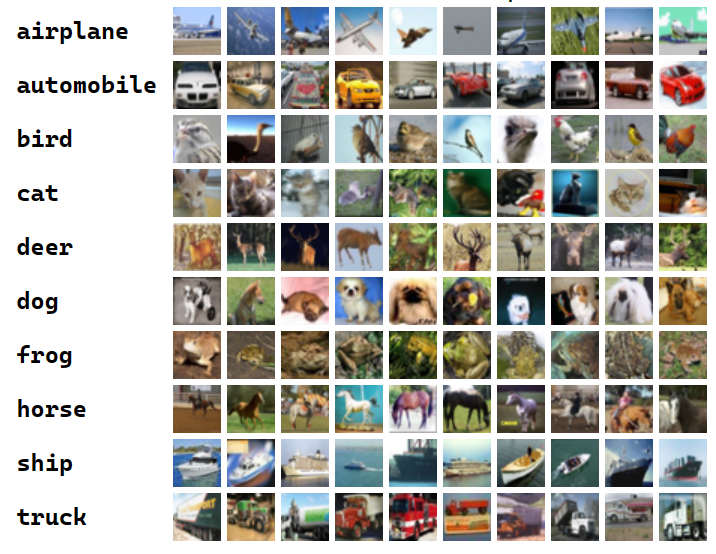
\includegraphics[width=0.9\linewidth]{figure/cifar}
\caption{Ten randomly select images from 10 classes.}
\label{fig:cifar}
\end{figure}

In this project, I will directly use the datasets provided in the \texttt{torchvision} library, which is part of the PyTorch deep learning framework. Torchvision is a library consists of lots of datasets (including MNIST, CIFAR-10, ImageNet, ...) and pretrained model (including ResNet, VGGNet, BERT, ...).

As for the test set, I will use the original train/test split of the CIFAR-10 datasets. The datasets is divided into 50,000 training images and 10,000 testing images, with an equal number of images from each class in both sets. This train/test split is commonly used in the literature and provides a fair evaluation of the performance of machine learning models on the CIFAR-10 datasets.

It's also worth noting that cross validation can be also used for the CIFAR-10 datasets. However, the number of images in the datasets is large and most of the research paper use the original train/test split. Therefore, it's reasonable for this project to use the original train/test split.

Noted that I also use torchvision to download and process the datasets.

\subsection{Algorithms}

For the CIFAR-10 datasets, I use two classifier, ResNet-18 and Multilayer Perceptron (MLP).

\subsubsection{ResNet-18}

ResNet-18 is a popular deep convolutional neural network architecture used for image classification tasks. It was introduced by Microsoft Research in 2015 and is part of a family of ResNet models, which are designed to tackle the problem of vanishing gradients in very deep neural networks. ResNet has different variance, from ResNet-18 all the way to ResNet-152. The number after ResNet indicates the number of layers. Therefore, ResNet-18 is a relatively shallow model, with 18 layers, but it still achieves state-of-the-art performance on a range of image classification benchmarks, including ImageNet, CIFAR-10, and CIFAR-100.

For the sake of convenience, I directly use the ResNet-18 models which provides in torchvision library. Torchvision library also provides the pretrained weights. However, those weights are trained on ImageNet Datasets, not CIFAR-10. Therefore, I also compare the performance with or without using pretrained weights. There are more details in appendix.

It's worth noting that because the image size of CIFAR-10 is only 32 x 32. And ResNet is original designed for ImageNet, which image size is 224 x 224. Therefore, the first convolution layer with kernel size equals to 7 is too large for CIFAR-10 datasets, this will make lots of features lost from the first convolution layer. Moreover, the max pooling layer may also make features lost. Therefore, I change the kernel size from 7 to 3 and  also remove the max pooling layer. In the analysis section, I will discuss the performance difference after changing these two layers.

\subsubsection{MLP}

A multilayer perceptron (MLP) is a type of artificial neural network (ANN) that consists of multiple layers of interconnected nodes (also called neurons) in a feedforward network architecture. It is one of the most commonly used neural network models for supervised learning tasks such as classification, regression, and pattern recognition.


An MLP typically consists of an input layer, one or more hidden layers, and an output layer. The number of neurons in the input layer is determined by the number of features in the input data, while the number of neurons in the output layer corresponds to the number of output classes or the number of output variables in a regression task. The number of neurons in the hidden layers is a hyperparameter that can be tuned during the training process.

We know that MLP has one input layer, one output layer and several hidden layers. In this project, I will only use an MLP that consists of two hidden layers with same number of neurons. The number of neurons is also a hyperparameters that will compare in the analysis section. As for the input layer, I just flatten the images into an one dimensional vector, with $3 \times 32 \times 32 = 3072$ elements as input. For the output layer, MLP will output a one dimensional vector with 10 elements, corresponding to 10 classes.

\subsubsection{Epochs, Loss Function, Optimizer and Learning Rate Scheduler}

In the following experiments, I will use the below configuration for both MLP and ResNet-18. 

\begin{itemize}
\item Epochs: 200
\item Learning Rate: 0.1
\item Loss Function: \texttt{CrossEntropyLoss}
\item Optimizer: \texttt{SGD}
\item Learning Rate Scheduler: \texttt{ReduceLROnPlateau} (monitor on \texttt{val\_acc, patient=10, factor=0.1})
\item Batch Size: 128
\end{itemize}

Learning rate scheduler is a tool to change learning rate while training. And the LR scheduler I use will monitor on \texttt{val\_acc}. When \texttt{val\_acc} doesn't increase for 10 epochs, the learning rate will be reduced by 90\%.

\subsection{Analysis}

First of all, because CIFAR-10 already has provided a train/test split, I will not use cross-validation for this datasets.

\subsubsection{Compare Different Architecture of ResNet-18}

As I mentioned earlier, because the kernel size of first convolution layer is too large for images in CIFAR-10 datasets, I change the kernel size and also remove the first max pooling layer. This version is called ``Modified ResNet-18'', and the unmodified one is called ``Original ResNet-18''. As we can see in the chart from \autoref{chart: res_1} to \autoref{chart: res_4}, the modified one is significant better than the unmodified one. The highest test accuracy for the modified one is 0.9227, in the contrast, the unmodified one is 0.8766.

In conclusion, changing the architecture of ResNet can indeed significantly improve the model's accuracy.

\subsubsection{Comparing whether there is a pre-trained weight for ResNet-18}\label{sec: pre-trained}

PyTorch provides a pretrained weight for ResNet-18. However, the pretrained weight is trained on ImageNet datasets. Therefore, it might perform well on CIFAR-10 datasets. Because of this I make an experiment to test how the existence of pretrained weight affect the performance of model.

As we can see in \autoref{chart:resnet-18-cifar-10-pretrained-acc} and \autoref{chart:resnet-18-cifar-10-pretrained-loss}, the ResNet-18 with pretrained weight doesn't perform very well. The highest test accuracy of ResNet-18 without pretrained weight is 0.9227, as for the model with pretrained weight, this number is 0.9177. I will discuss more in \ref{sec: discuss-1}.

\subsubsection{Compare Different Architecture of MLP}

For the MLP, I fixed the number of hidden layer to two. And by setting the number of neurons in hidden layers to 100 and 2500, I trained two MLP model.

As we can see in the chart (\autoref{chart: mlp_1} to \autoref{chart: mlp_4}), the MLP with 2500 hidden neurons is significant better than the 100 ones. The highest testing accuracy for the 2500 one is 0.5886, as for the 100 ones is 0.5324.

\subsubsection{Compare Different Amount of Training Data}

In this section, I will first analysis ResNet-18 case, and then analysis MLP case. 

Noted that though the number of training data is different, the testing data for both model is exactly the same.

First, for ResNet-18, we can look at \autoref{fig:resnet-half-cifar-acc} and \autoref{fig:resnet-half-cifar-loss}. As we can observe, the ``half'' one train much more slower than the ResNet-18 that trained with full training CIFAR-10 datasets, which contains 50000 images. And the final test accuracy, the ``half'' one's accuracy is 0.8782. Which is less than the full-trained model by around 5\%.

Second, let's look at the MLP. Also we can observe that in \autoref{fig:mlp-half-cifar-acc} and \autoref{fig:mlp-half-cifar-loss}, the training accuracy of the MLP with full training datasets is slightly better, and for the testing accuracy, it is nearly the same. The ``Half MLP'' is 0.5816, and the ``Full MLP`` is 0.5886.

\subsubsection{Compare with SOTA Model}

After researching, the state-of-the-art model on CIFAR-10 is Vision Transformer (ViT). In particularly, the ViT-H/14 model can achieve 99.5\% test accuracy, which is astonishing results. However, this model require 632M parameters, in the contrast, ResNet-18 only requires 11M parameter.

In conclusion, ViT is 57 times larger than ResNet-18, but it only increase 7\% of accuracy.

\subsubsection{Overall Comparison}

From the above comparing, we know that the best performance for ResNet-18 is the modified ResNet-18 without pretrained weights. As for MLP, the best model is with 2500 hidden neurons. And the SOTA model for CIFAR-10 is ViT-H/18. 

For the overall comparison table, please refer to \autoref{table: cifar-table}.

\subsection{Discussion}

\subsubsection{Assessing Expected Results and Behaviors in Experiments}\label{sec: discuss-1}

\begin{enumerate}
\item \textbf{Using pretrained weights or not}

In \ref{sec: pre-trained}, I compare the performance of the ResNet-18 with or without pretrained weights. And the result is the model without pretrained weights has better performance.

One can guess the model with pretrained weights might be better, but it's not. I think one main reason is that I already changed the model architecture, therefore the idea of ``transfer learning'' didn't work well here. And also, the distribution of CIFAR-10 and ImageNet is also difference. Therefore, trained the model from scratch might be a better idea.

In conclusion, I think these are the two main reasons why the model without pretrained weights is better.

\end{enumerate}

\subsubsection{Factors Affecting Performance}

\begin{enumerate}
\item Model architecture
\item Different hyperparameters
\item Number of epochs count
\item Number of training data
\item LR scheduler

Using LR scheduler is actually really important for machine learning, especially when SGD is used. Because larger LR in the later stage of training might make the model can't converge to optimal point. Therefore it's necessary to have LR scheduler.
\end{enumerate}

\subsubsection{Future Experiments}

\begin{enumerate}
\item \textbf{Using adam optimizer instead of SGD.}

The adam optimizer can change the learning rate of each weights, which is might be a better method compared with LR decay. The SGD along with LR decay method may take longer time to converge.
\item \textbf{Apply features extractions before sending into MLP.}

Apply features extractions on images can extract useful features, and using these extracted features might be able to improve the MLP performance.
\end{enumerate}

\subsubsection{Findings and Open Questions from Experiments}

\begin{enumerate}
\item \textbf{MLP doesn't perform very well}

Before conducting the experiment, I thought it may achieve an accuracy around 70\%. But it turns out only get 60\%.

\item \textbf{Changing the architecture of the CNN is useful}

I improved the model's accuracy by 5\% by only changing the kernel size of one layer and removing one max pooling layer. This is a new inspiration for me that sometimes we need to compare the difference of the images we need to classify now with the designated image, and based on the input images to design the proper architecture. 
\end{enumerate}

\section{Public Non-Image Datasets: 20 Newgroups}
\subsection{Datasets Description}

The 20 Newsgroups datasets is a popular datasets used in natural language processing and machine learning research. It consists of a collection of approximately 20,000 documents, partitioned into 20 different newsgroups, each representing a different topic. The datasets was first collected by Ken Lang and others at the University of California, Irvine, and has since been widely used in research and experimentation.

Each document in the 20 Newsgroups datasets is a posting to one of the 20 newsgroups, and is represented as a single text file. The datasets includes a variety of topics, including politics, religion, sports, science, and technology, among others.

In this project, I will use vectorize version of this datasets. This is done by using the \texttt{CountVectorize} in scikit-learn library. In this way, the text data is transformed to real-valued vector, which can be processed by \texttt{RandomForestClassifier}, \texttt{GradientBoostingClassifier}, \texttt{AdaBoostClassifier}, etc.

\subsection{Algorithms}

In this datasets, I use four kinds of ensemble learning algorithms, Random Forest Classifier, Gradient Boosting Classifier, Histogram-based Gradient Boosting Classifier and AdaBoost Classifier. One SVM algorithm, linear SVM. And a MLP Classifier, which is same MLP architecture in the first datasets. Therefore, I will only talk about the four ensemble learning algorithms and the SVM algorithm.

Random Forest Classifier, Gradient Boosting Classifier, Histogram-based Gradient Boosting Classifier and AdaBoost Classifier are all powerful machine learning algorithms commonly used for classification tasks. These algorithms are known for their ability to handle complex datasets and provide accurate predictions.

And SVM (Support Vector Machines) is also a machine learning algorithm used for classification and regression analysis. It was developed by Vapnik and his colleagues in the 1990s. SVM is a supervised learning algorithm that works by finding the optimal hyperplane that separates the data into different classes. The hyperplane is chosen in a way that maximizes the margin between the closest data points from each class. These closest data points are known as support vectors.

These six classifiers can be found in the \texttt{scikit-learn} library. In the following experiments, I directly apply the default value of \texttt{scikit-learn} provides. I state the option clearly in different classifier.

\subsubsection{Random Forest Classifier}

Random Forest Classifier is an ensemble learning algorithm that creates multiple decision trees and combines their outputs to make a final prediction. Each tree is trained on a random subset of the features and samples of the dataset, making the algorithm robust to overfitting. The final prediction is made by taking the mode of the predictions of all trees in the forest.

\begin{itemize}
\item The number of tree: 1000 or 500 (compare the difference)
\item Criterion: Gini Impurity
\end{itemize}

\subsubsection{Gradient Boosting Classifier}

Gradient Boosting Classifier is another ensemble learning algorithm that creates multiple weak learners and combines their outputs to make a final prediction. Unlike Random Forest Classifier, it creates trees sequentially, with each new tree correcting the errors of the previous tree. This iterative process continues until a stopping criterion is met, resulting in a strong learner that makes accurate predictions.

Gradient Boosting algorithm is widely used in many machine learning competitions in Kaggle. This is reason why I choose this algorithms in this project.

\begin{itemize}
\item The Number of Tree: 100 or 50 (compare the difference)
\item Loss Function: \texttt{log\_loss}
\item Criterion: \texttt{friedman\_mse}
\item Learning Rate: 0.1
\item Max Depth: 3
\end{itemize}

\subsubsection{Histogram-based Gradient Boosting Classifier}

The Histogram-based Gradient Boosting Classifier is a variation of the standard gradient boosting classifier in scikit-learn. The primary difference between the two lies in the way they handle large datasets.

The traditional gradient boosting classifier typically uses the entire dataset to build the decision tree at each boosting iteration. This can be computationally expensive and slow for large datasets. In contrast, the Histogram-based Gradient Boosting Classifier uses histogram-based gradient boosting, which aggregates and precomputes information about the dataset in bins or buckets, making it more efficient for large datasets.

Furthermore, the Histogram-based Gradient Boosting Classifier uses a technique called gradient-based early stopping, which allows it to automatically stop training once the model starts to overfit the training data. This is different from the traditional gradient boosting classifier which requires the user to manually specify the number of boosting iterations.

Overall, while the standard gradient boosting classifier is a powerful algorithm that can produce accurate predictions, the Histogram-based Gradient Boosting Classifier is a more efficient and scalable algorithm that is particularly useful for large datasets with high dimensionality.

The \texttt{scikit-learn} implementation is inspired by \href{https://github.com/Microsoft/LightGBM}{LightGBM}.

\begin{itemize}
\item Epoch: 100 or 50 (compare the difference)
\item Loss Function: \texttt{log\_loss}
\item Learning Rate: 0.1
\item Maximum Leaf Nodes: 31
\item Maximum Number of Bins: 255
\item Tolerance: $10^{-7}$
\item Patience: 10
\end{itemize}

\subsubsection{AdaBoost Classifier}

AdaBoost Classifier, short for Adaptive Boosting Classifier, is also an ensemble learning algorithm that creates multiple weak learners and combines their outputs to make a final prediction. It is similar to Gradient Boosting Classifier in that it creates trees sequentially, but it assigns weights to each sample in the datasets based on how difficult it is to classify correctly. Samples that are misclassified by a weak learner are given higher weights, making them more likely to be correctly classified by the next weak learner.

\begin{itemize}
\item Estimator: Decision tree with maximum depth 1
\item Number of Estimators: 50 or 500 (compare the difference)
\item Algorithm: SAMME.R
\end{itemize}

\subsubsection{Linear SVM Classifier}

Linear SVM is a specific type of SVM that assumes the data is linearly separable, meaning that a straight line can be drawn to separate the data points into different classes. Linear SVM is used when the data is linearly separable, which means that the data can be classified into two or more classes by a straight line. In this case, the SVM algorithm finds the optimal hyperplane in a way that maximizes the margin between the closest data points from each class while keeping the classification error rate as low as possible.

Linear SVM is a simple and effective algorithm that works well on a wide range of problems. However, it may not work well when the data is not linearly separable. In this case, other types of SVMs or non-linear methods may be more appropriate.

\begin{itemize}
\item Penalty: L2
\item Loss: squared hinge
\item dual: True or False (compare the difference)
\end{itemize}

\subsubsection{MLP Classifier}

Noted that this MLP Classifier is the built-in version in scikit-learn.

\begin{itemize}
\item Epochs: 200
\item Optimizer: Adam
\item Learning Rate: 0.001
\item Momentum: 0.9
\item Loss Function: \texttt{CrossEntropyLoss}
\item Tolerance: 0.0001
\item Patient: 10
\item Number of hidden layer: 1
\item Number of hidden neurons: 100
\end{itemize}

\subsection{Analysis}

\subsubsection{Compare Different Random Forest Classifier}
\subsubsection{Compare Different Gradient Boosting Classifier}
\subsubsection{Compare Different Histogram-based Gradient Boosting Classifier}
\subsubsection{Compare Different AdaBoost Classifier}
\subsubsection{Compare Different MLP Classifier}
\subsubsection{Compare Different Amount of Training Data}
\subsubsection{Compare with SOTA Model}

Currently, to my best knowledge, the SOTA of 20 newsgroups datasets is \href{https://arxiv.org/abs/2211.02563v1}{LinearSVM+TFIDF}. TFIDF is a kind of vectorizer and LinearSVM is just a simple SVM algorithm.

\subsubsection{Overall Comparison}

\subsection{Discussion}
\subsubsection{Assessing Expected Results and Behaviors in Experiments}

Before conducting the experiment, I guess the Adaboost or histogram-based gradient boosting algorithm may perform pretty well. Because I heard that GB algorithms perform really well on lots of Kaggle competition. However, after the experiments, I found that the best model is simple linear SVM classifier, and it only took around 2 minutes to finished training. Compared to histogram-based gradient boosting, it takes nearly 40 minutes to binning the data, and 4.6 hours to train the model. Which is really time-consuming, and the result is not really good. This really surprised me. I will have more research on this behavior after this project.

\subsubsection{Factors Affecting Performance}

\begin{enumerate}
\item Different algorithms
\item The latent distribution of data
\item Different vectorizer and preprocessing method
\end{enumerate}

\subsubsection{Future Experiments}

\begin{enumerate}
\item \textbf{Try to use different vectorizer}
\item \textbf{Try more text preprocessing}

Including removing stop words, stemming, etc.

\item \textbf{Try to use NLP Model like BERT}
\end{enumerate}

\subsubsection{Findings and Open Questions from Experiments}

\begin{enumerate}
\item Linear SVM classifier is a great model for some cases
\item Histogram-based gradient boosting is time consuming
\item For simple classification task, the traditional machine learning can already perform really well
\end{enumerate}

\section{Self-made Datasets: Satellite Images of 5 Regions}
\subsection{Datasets Description}

In this datasets, I collect the satellite images of mountain area from 5 regions over the world, including Taiwan, Canada, Himalaya, Hengduan and Argentina. The task is to classify the satellite images to these five regions. The satellite images are from MapTiler, a tile map service. I first calculate which tiles should be download, then combine those tiles into a PNG file. Each image is an $256 \times 256$ RGB images.

\begin{figure}[H]
\centering
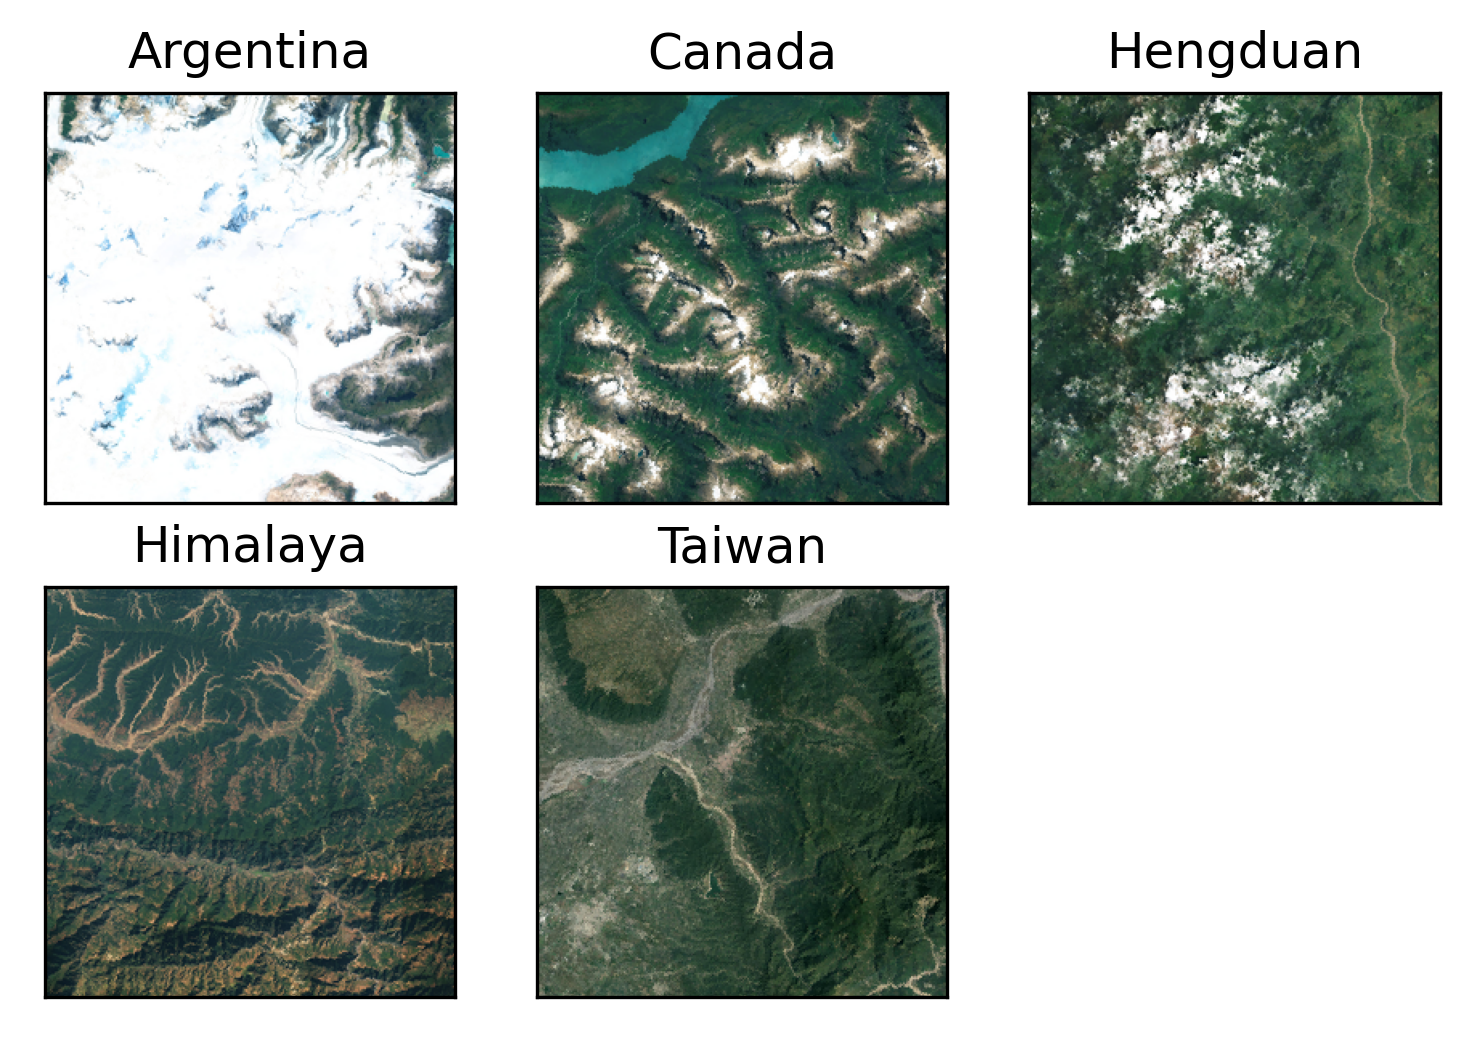
\includegraphics[width=0.9\linewidth]{figure/terrain_regions}
\caption{This figure shows 5 satellite images from 5 regions}
\label{fig:terrainregions}
\end{figure}

\subsection{Algorithms}

Because this datasets is also a image datasets, I just use the two classifiers (ResNet-18 and MLP) which used in the CIFAR-10 datasets with the exact same hyperparameters and configurations.

For MLP, because directly use $3 \times 256 \times 256$ as input layer is too large, I down-sampling the image from 256 x 256 to 128 x 128.

\subsection{Analysis}
\subsubsection{Compare Different Architecture of ResNet-18}
\subsubsection{Compare Different Architecture of MLP}
\subsubsection{Overall Comparison}

\subsubsection{Compare Different Amount of Training Data}

\subsubsection{Compare with SOTA Model}

\subsection{Discussion}
\subsubsection{Assessing Expected Results and Behaviors in Experiments}
\subsubsection{Factors Affecting Performance}
\subsubsection{Future Experiments}
\subsubsection{Findings and Open Questions from Experiments}


\clearpage
\pagenumbering{arabic}% resets `page` counter to 1
\renewcommand*{\thepage}{A. \arabic{page}}
\begin{appendices}
\section{Figures, Charts and Tables}

\subsection{Public Image Datasets: CIFAR-10}

\begin{figure}[H]
\centering
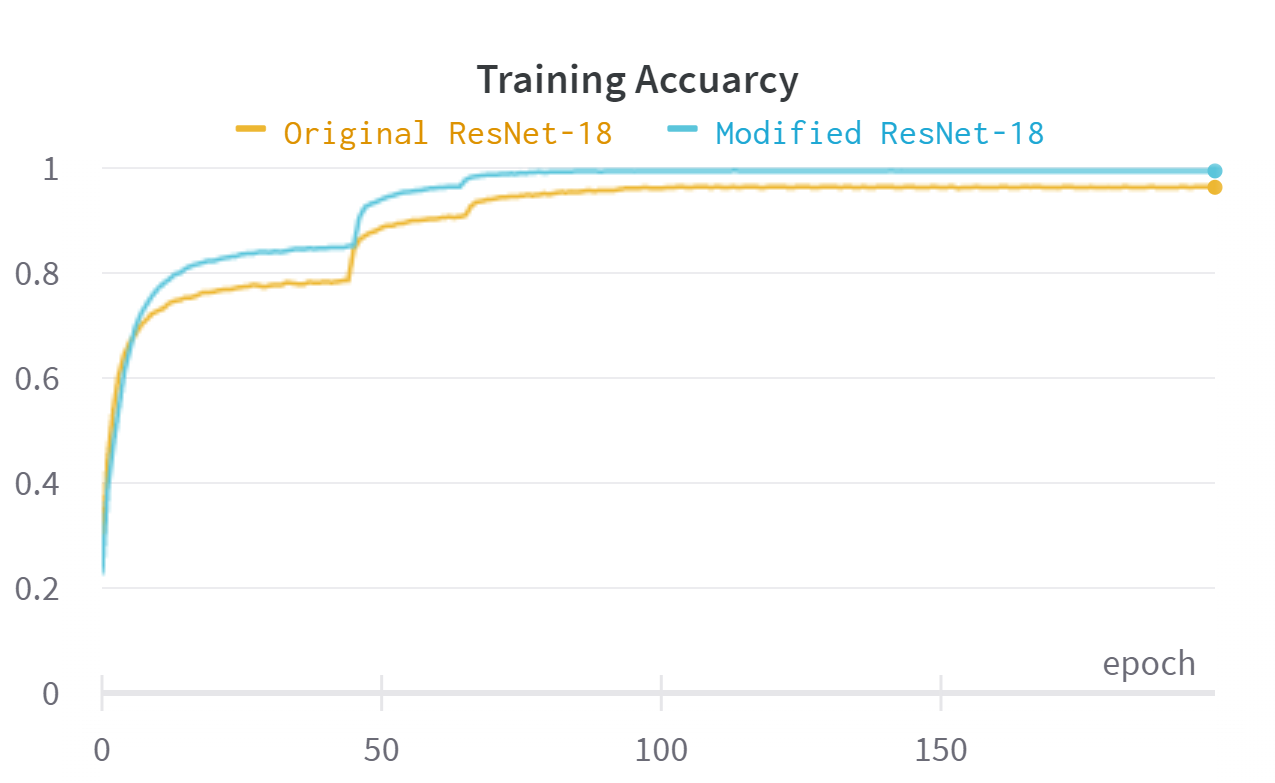
\includegraphics[width=0.9\linewidth]{charts/Section-2-Panel-0-uzzeut0la}
\caption{Training accuracy of two ResNet-18 models on CIFAR-10 datasets}
\label{chart: res_1}
\end{figure}

\begin{figure}[H]
\centering
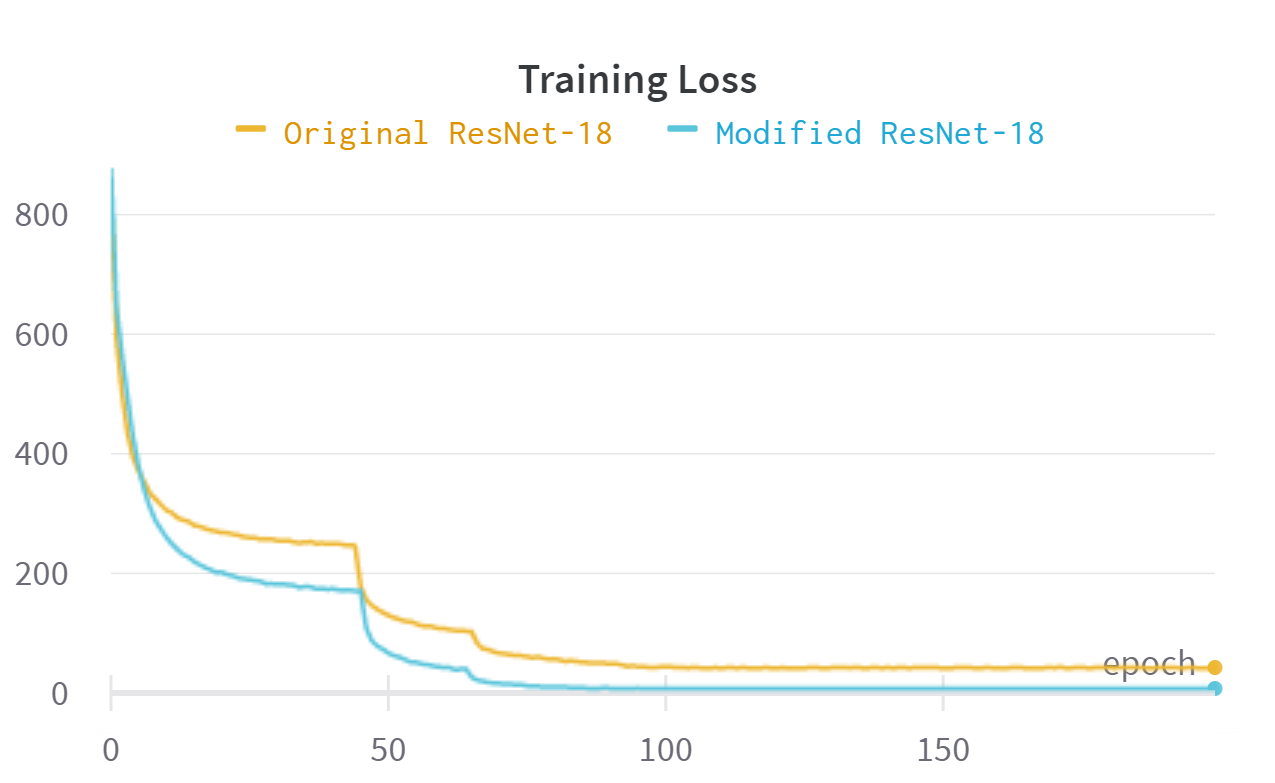
\includegraphics[width=0.9\linewidth]{charts/Section-2-Panel-1-crmf3l46q}
\caption{Training loss of two ResNet-18 models on CIFAR-10 datasets}
\label{chart: res_2}
\end{figure}

\begin{figure}[H]
\centering
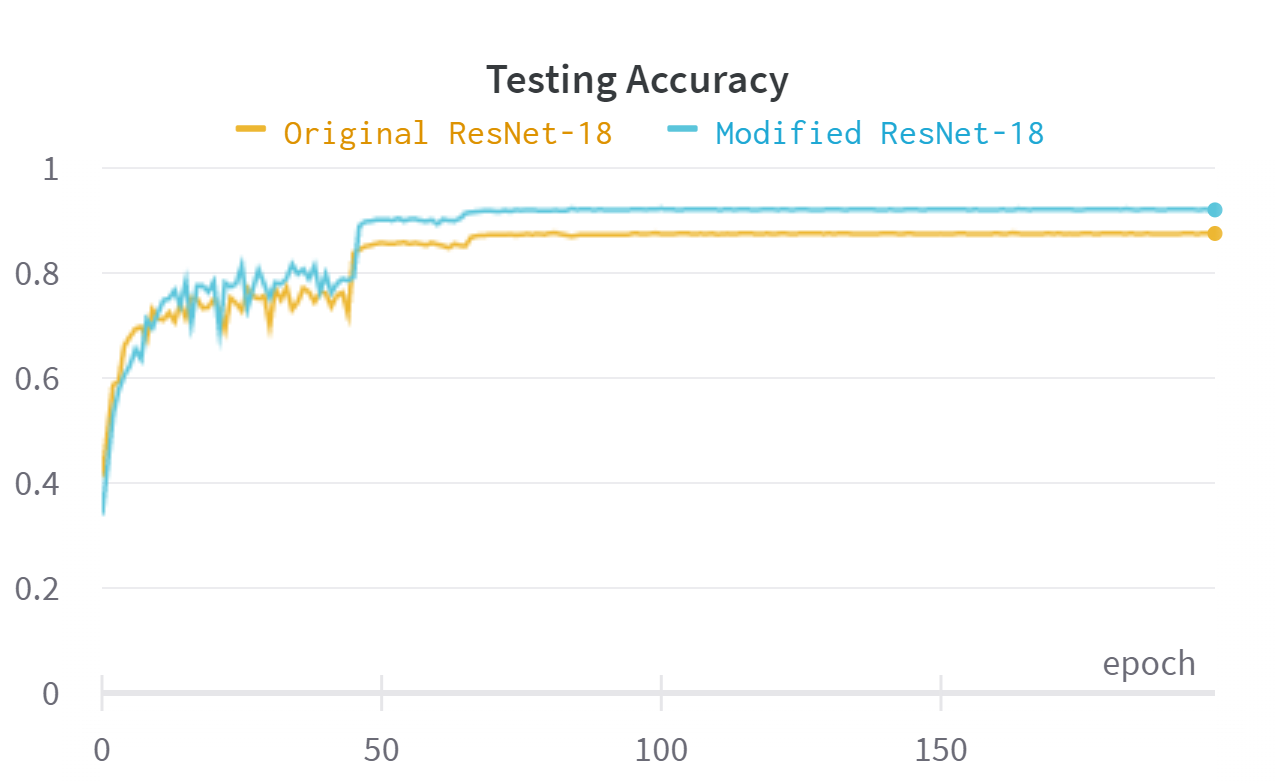
\includegraphics[width=0.9\linewidth]{charts/Section-2-Panel-2-qves7h50b}
\caption{Testing accuracy of two ResNet-18 models on CIFAR-10 datasets}
\label{chart: res_3}
\end{figure}

\begin{figure}[H]
\centering
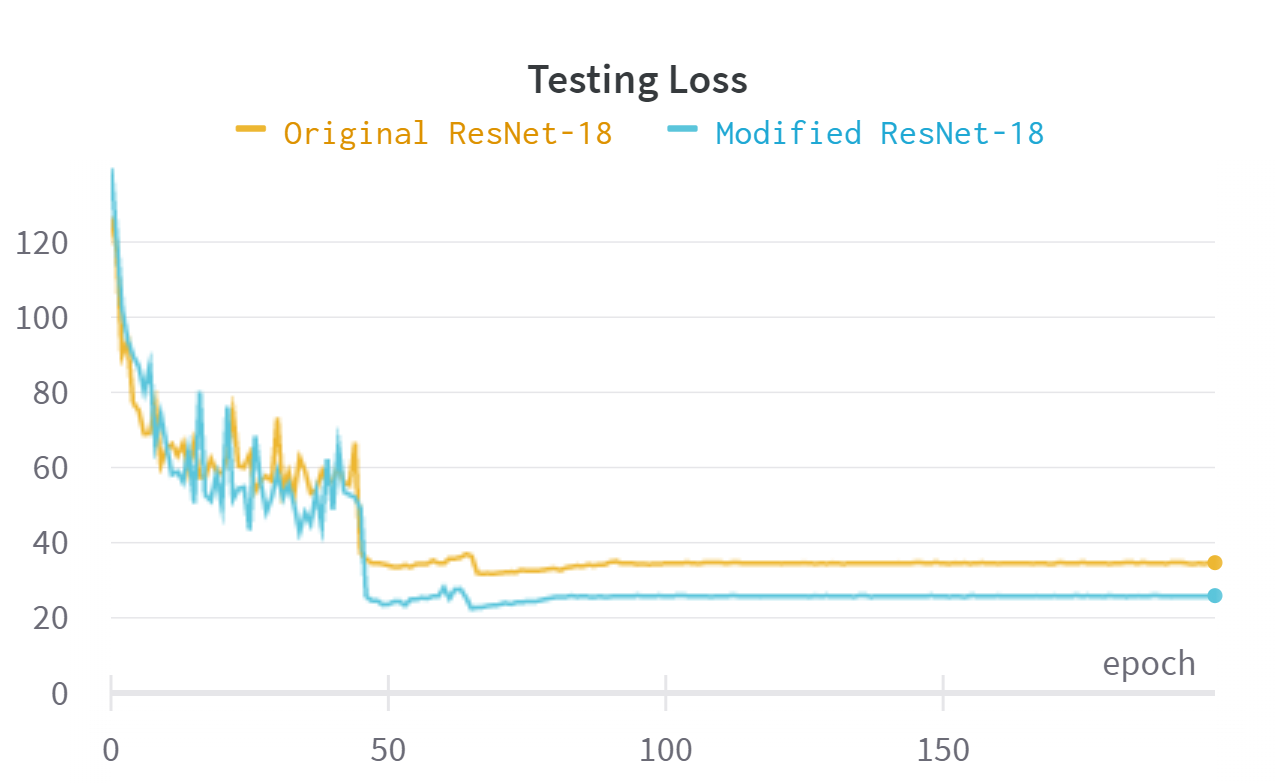
\includegraphics[width=0.9\linewidth]{charts/Section-2-Panel-3-cw0a3tnrd}
\caption{Testing loss of two ResNet-18 models on CIFAR-10 datasets}
\label{chart: res_4}
\end{figure}

\begin{figure}[H]
\centering
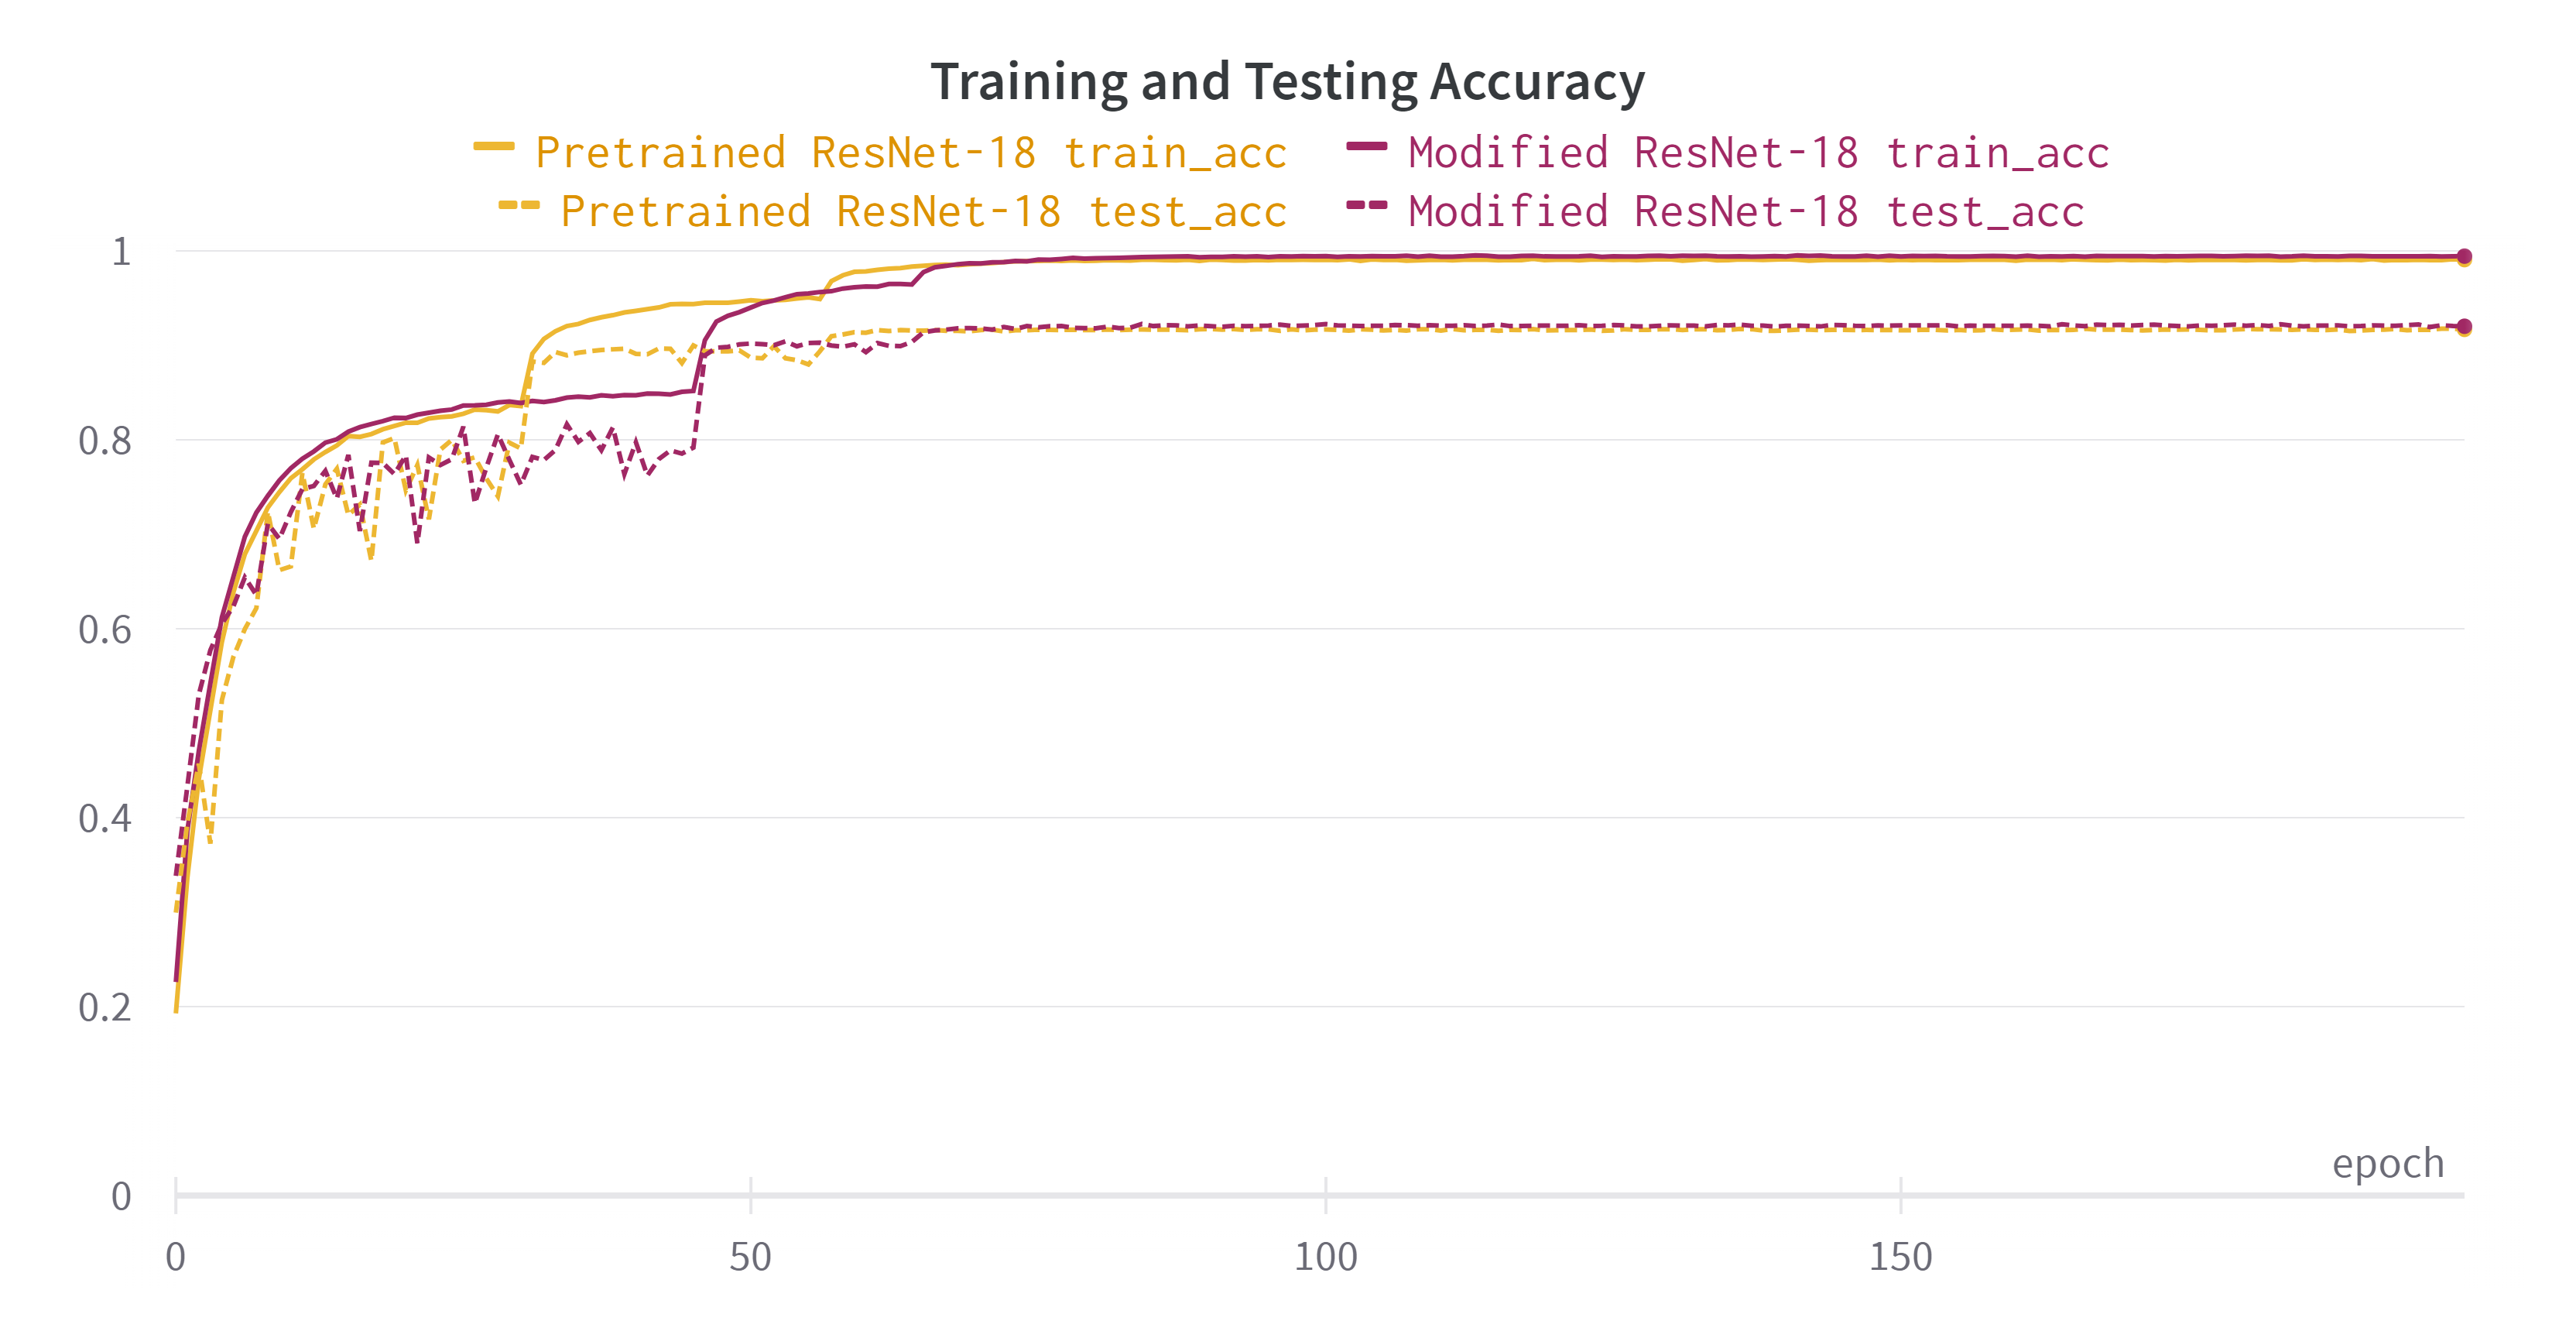
\includegraphics[width=0.9\linewidth]{charts/resnet-18-cifar-10-pretrained-acc}
\caption{Training and testing accuracy of two ResNet-18 model with and without ImageNet pretrained weight}
\label{chart:resnet-18-cifar-10-pretrained-acc}
\end{figure}

\begin{figure}[H]
\centering
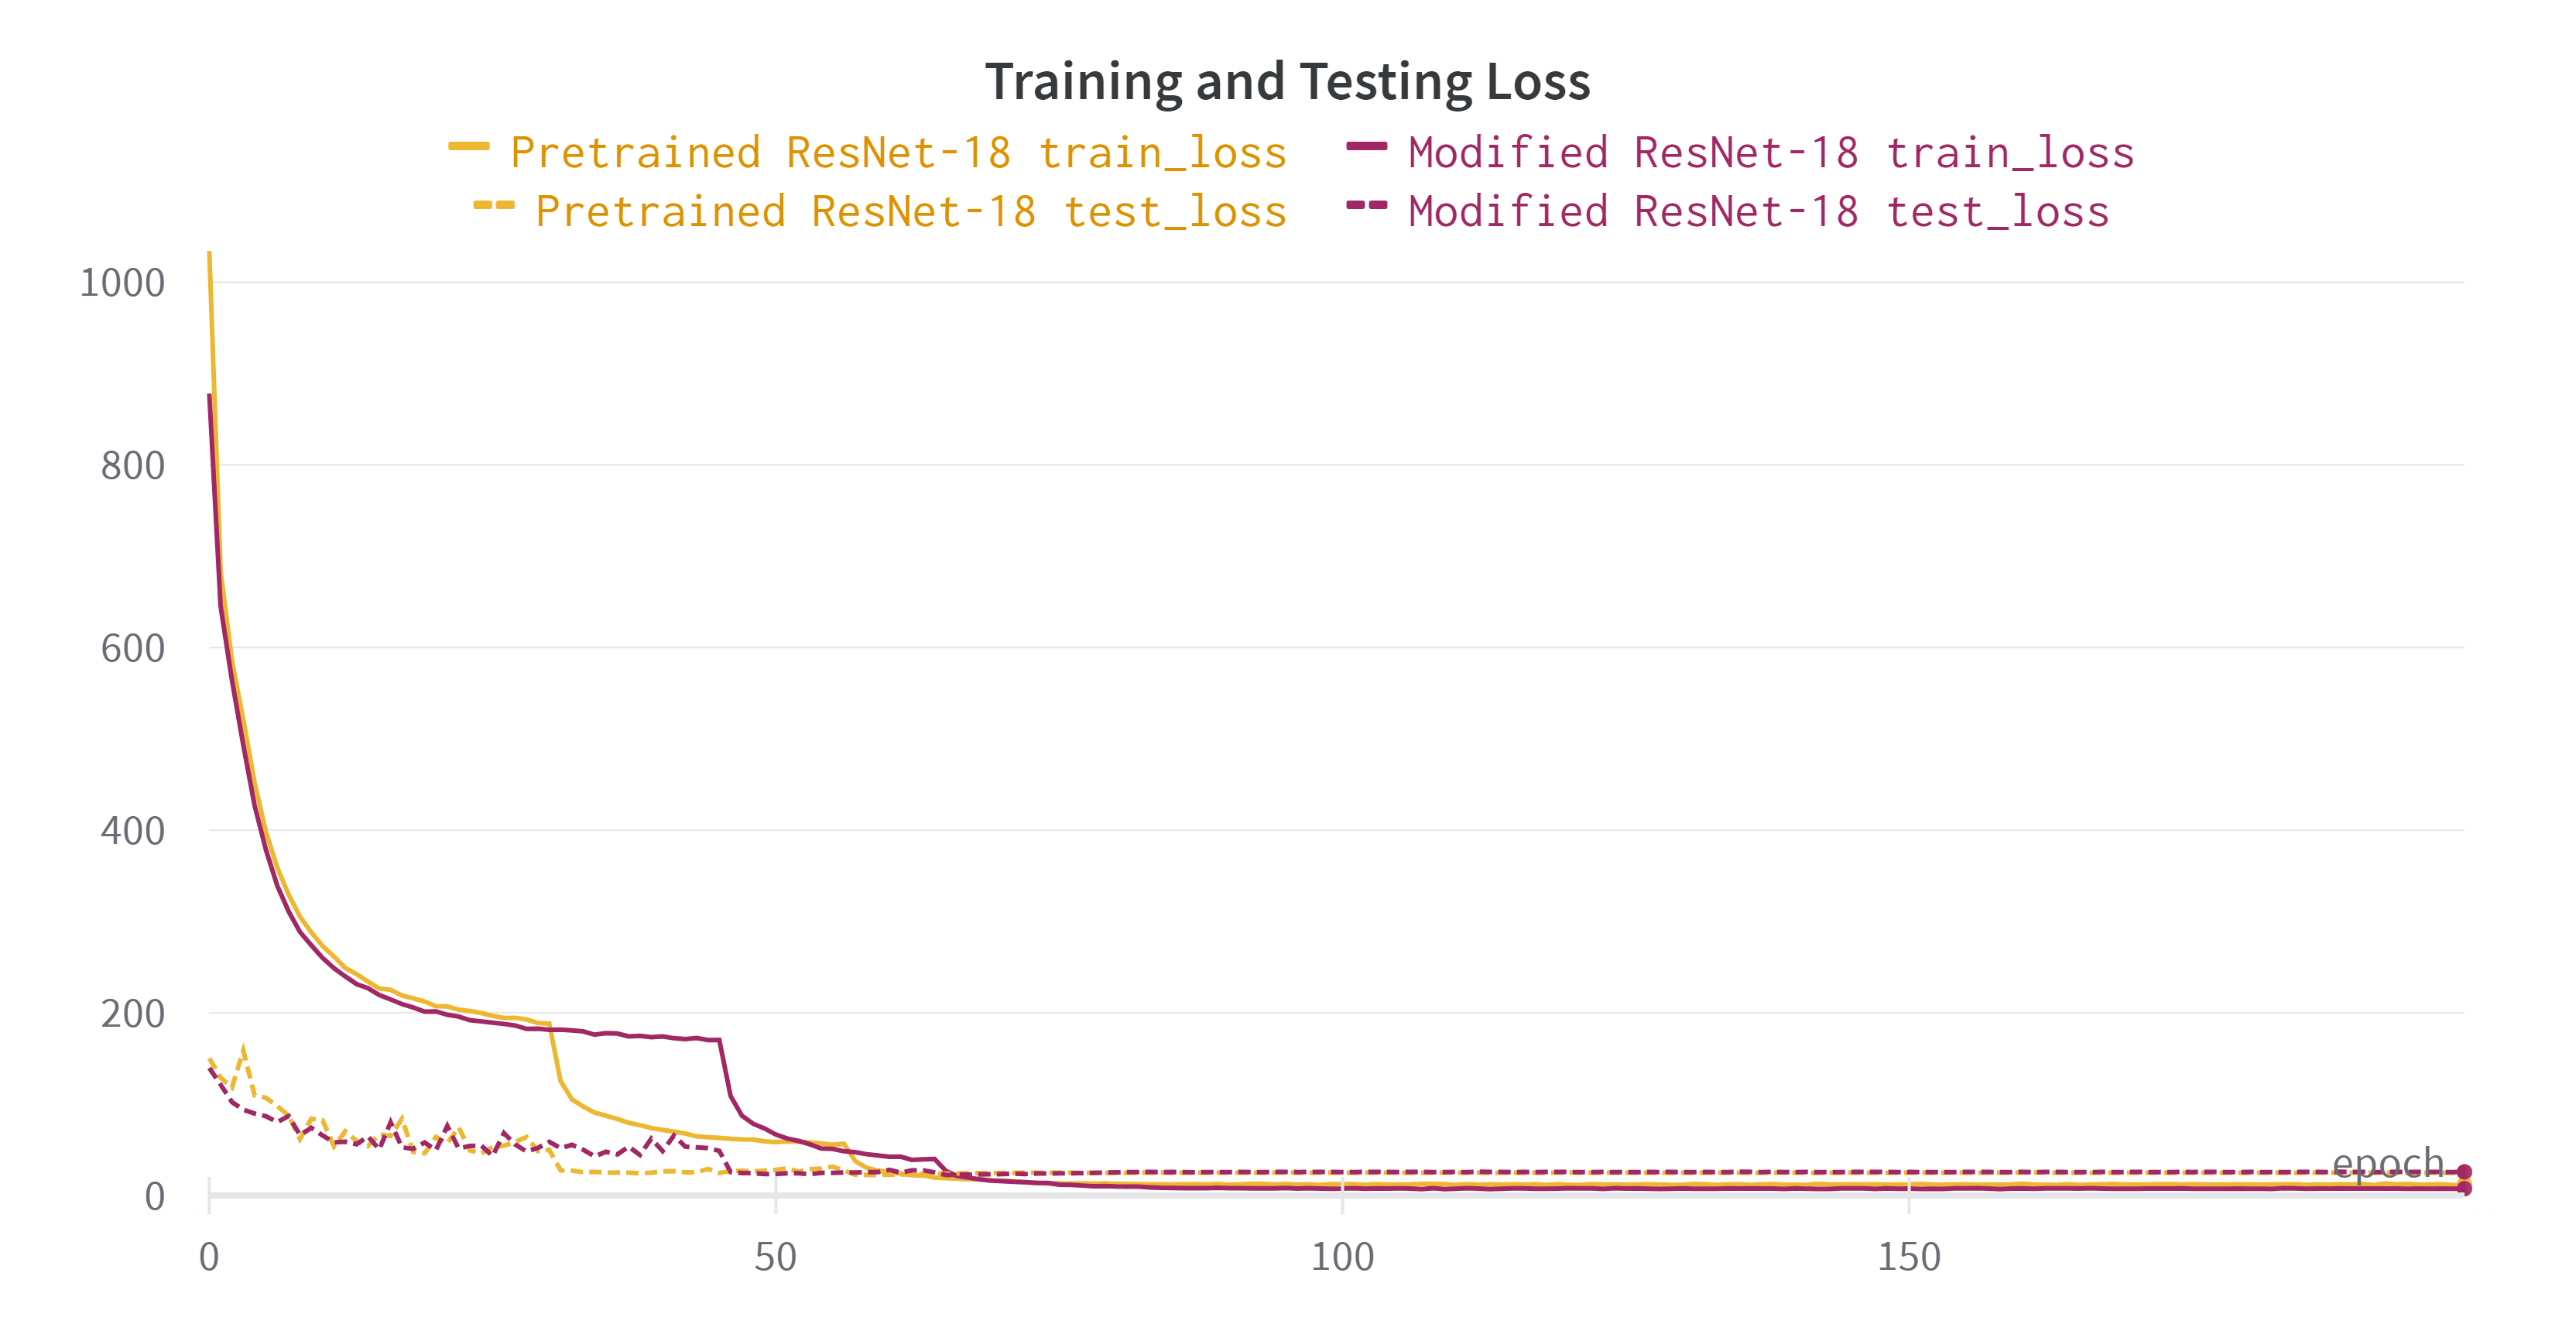
\includegraphics[width=0.9\linewidth]{charts/resnet-18-cifar-10-pretrained-loss}
\caption{Training and testing loss of two model with and without ImageNet pretrained weight}
\label{chart:resnet-18-cifar-10-pretrained-loss}
\end{figure}

\begin{figure}[H]
\centering
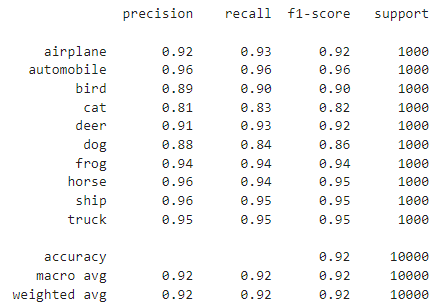
\includegraphics[width=0.9\linewidth]{charts/resnet-cifar-auc}
\caption{Accuracy table of pretrained ResNet-18}
\label{chart:resnet-cifar-auc}
\end{figure}

\begin{figure}[H]
\centering
\includegraphics[width=0.9\linewidth]{"charts/resnet-cifar-conf"}
\caption{Confusion matrix of pretrained ResNet-18}
\label{fig:resnet-cifar-conf}
\end{figure}

\begin{figure}[H]
\centering
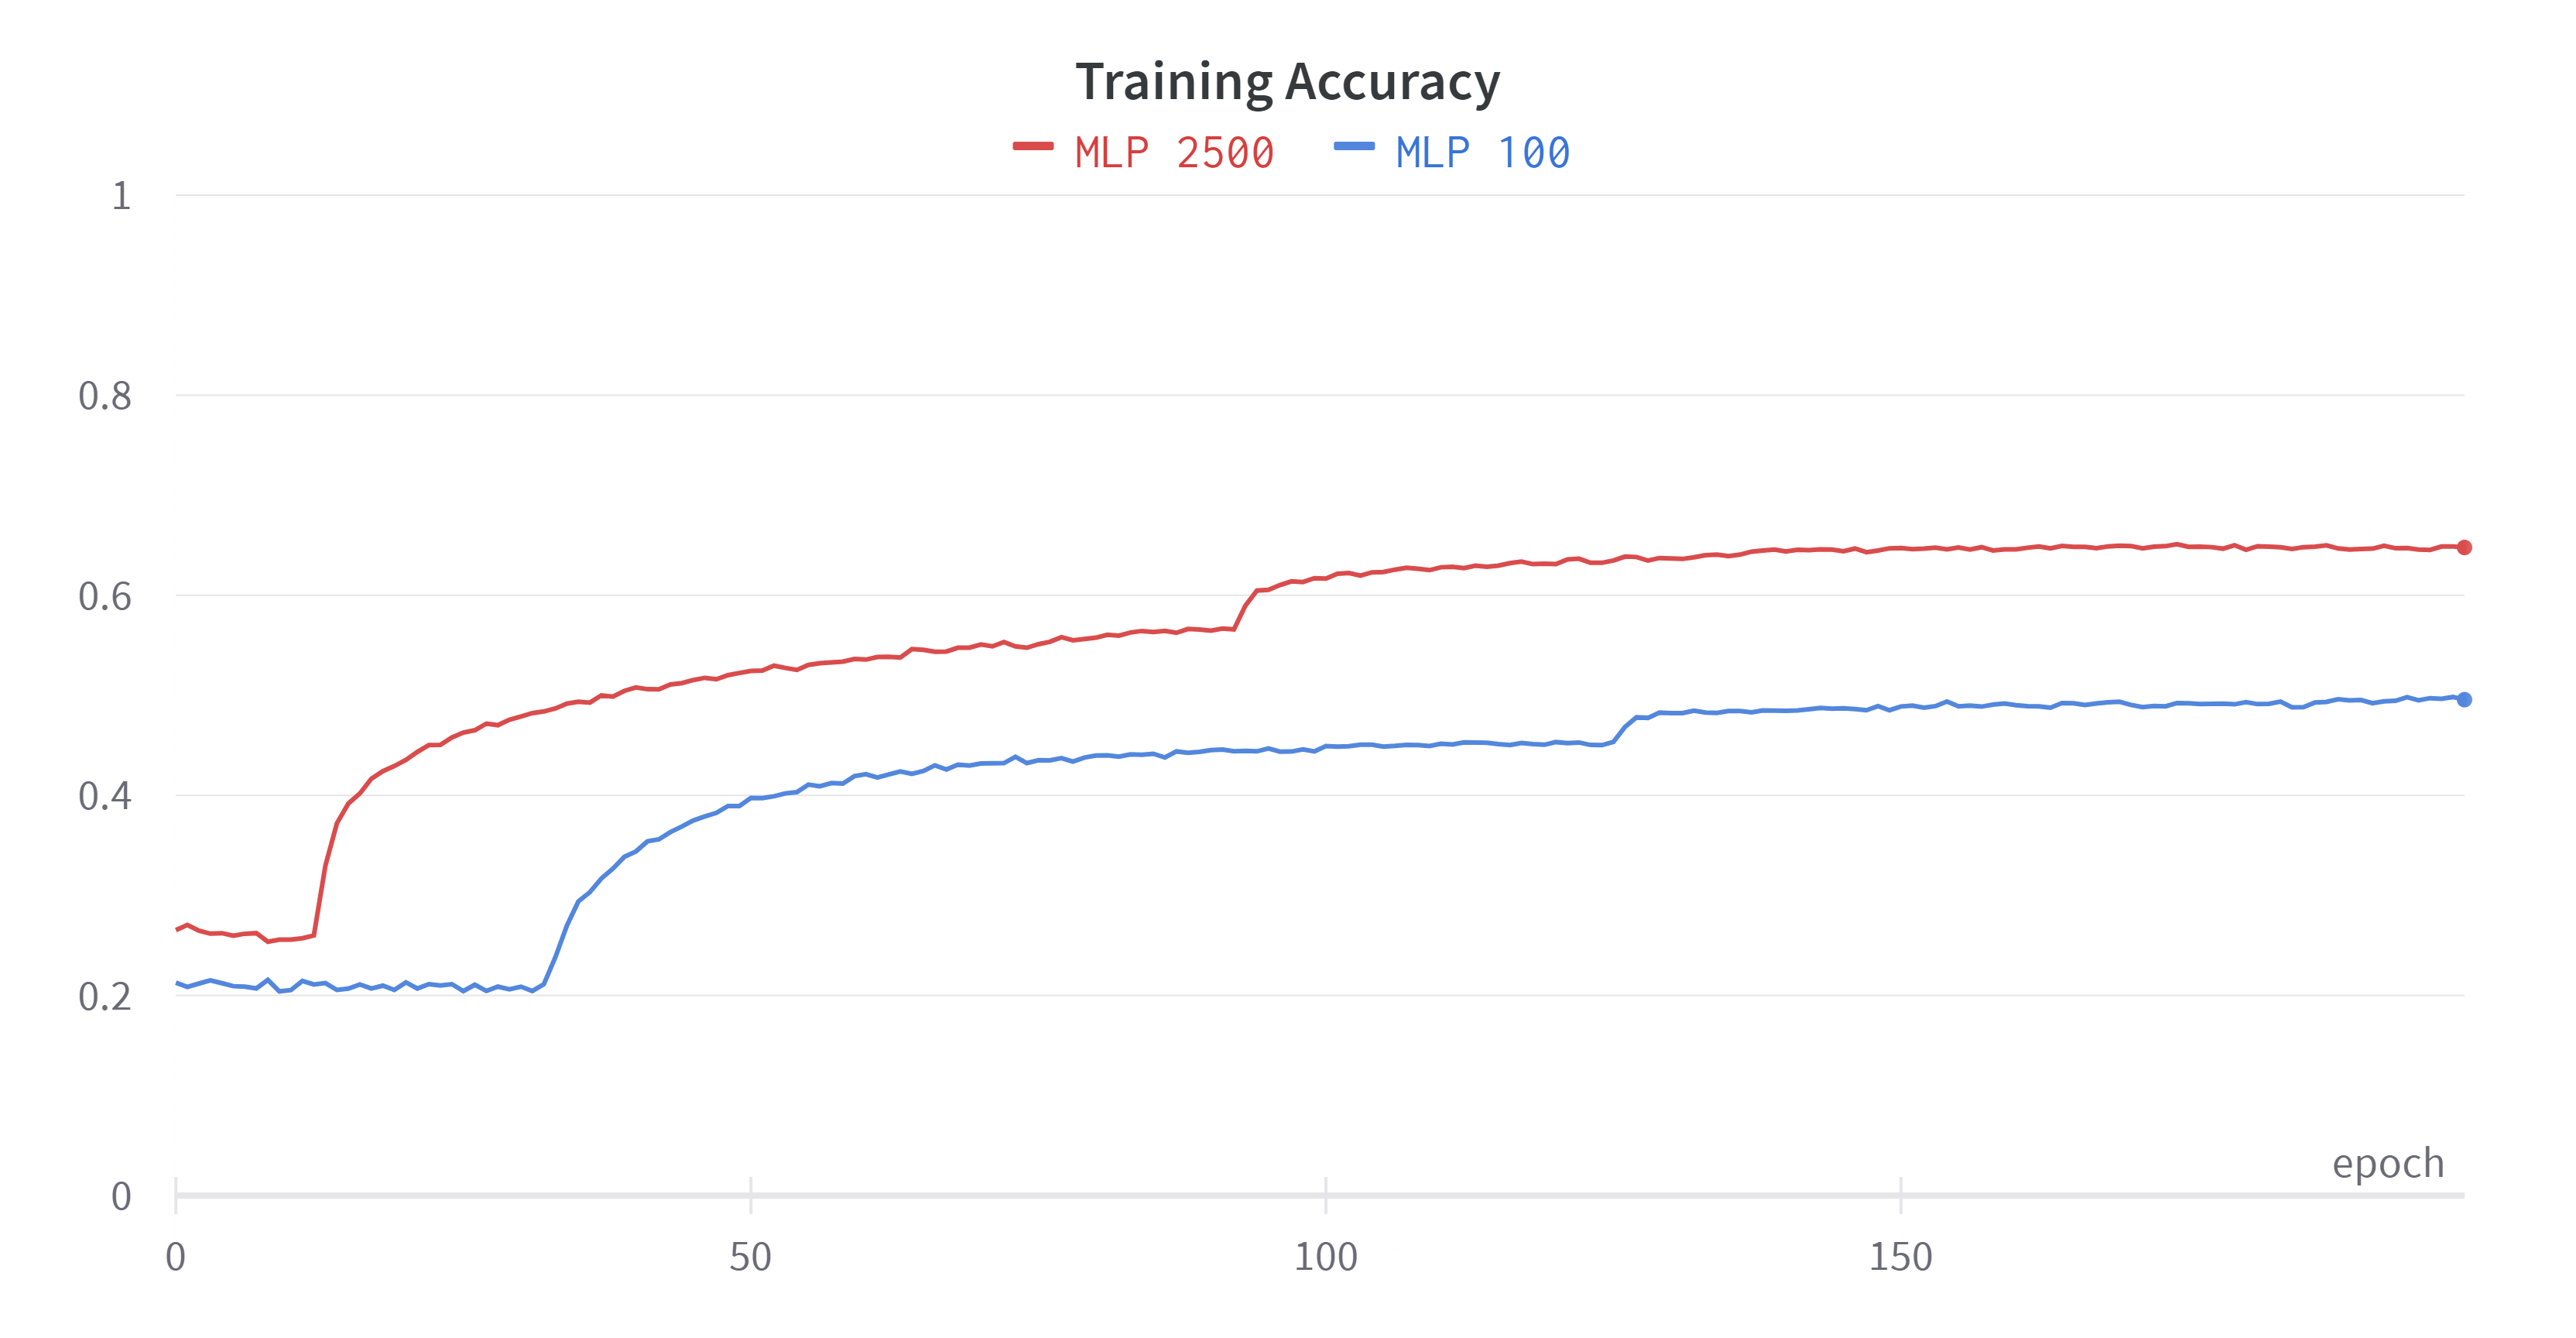
\includegraphics[width=0.9\linewidth]{charts/mlp_cifar_10_train_acc}
\caption{Training accuracy of two MLP models on CIFAR-10 datasets}
\label{chart: mlp_1}
\end{figure}

\begin{figure}[H]
\centering
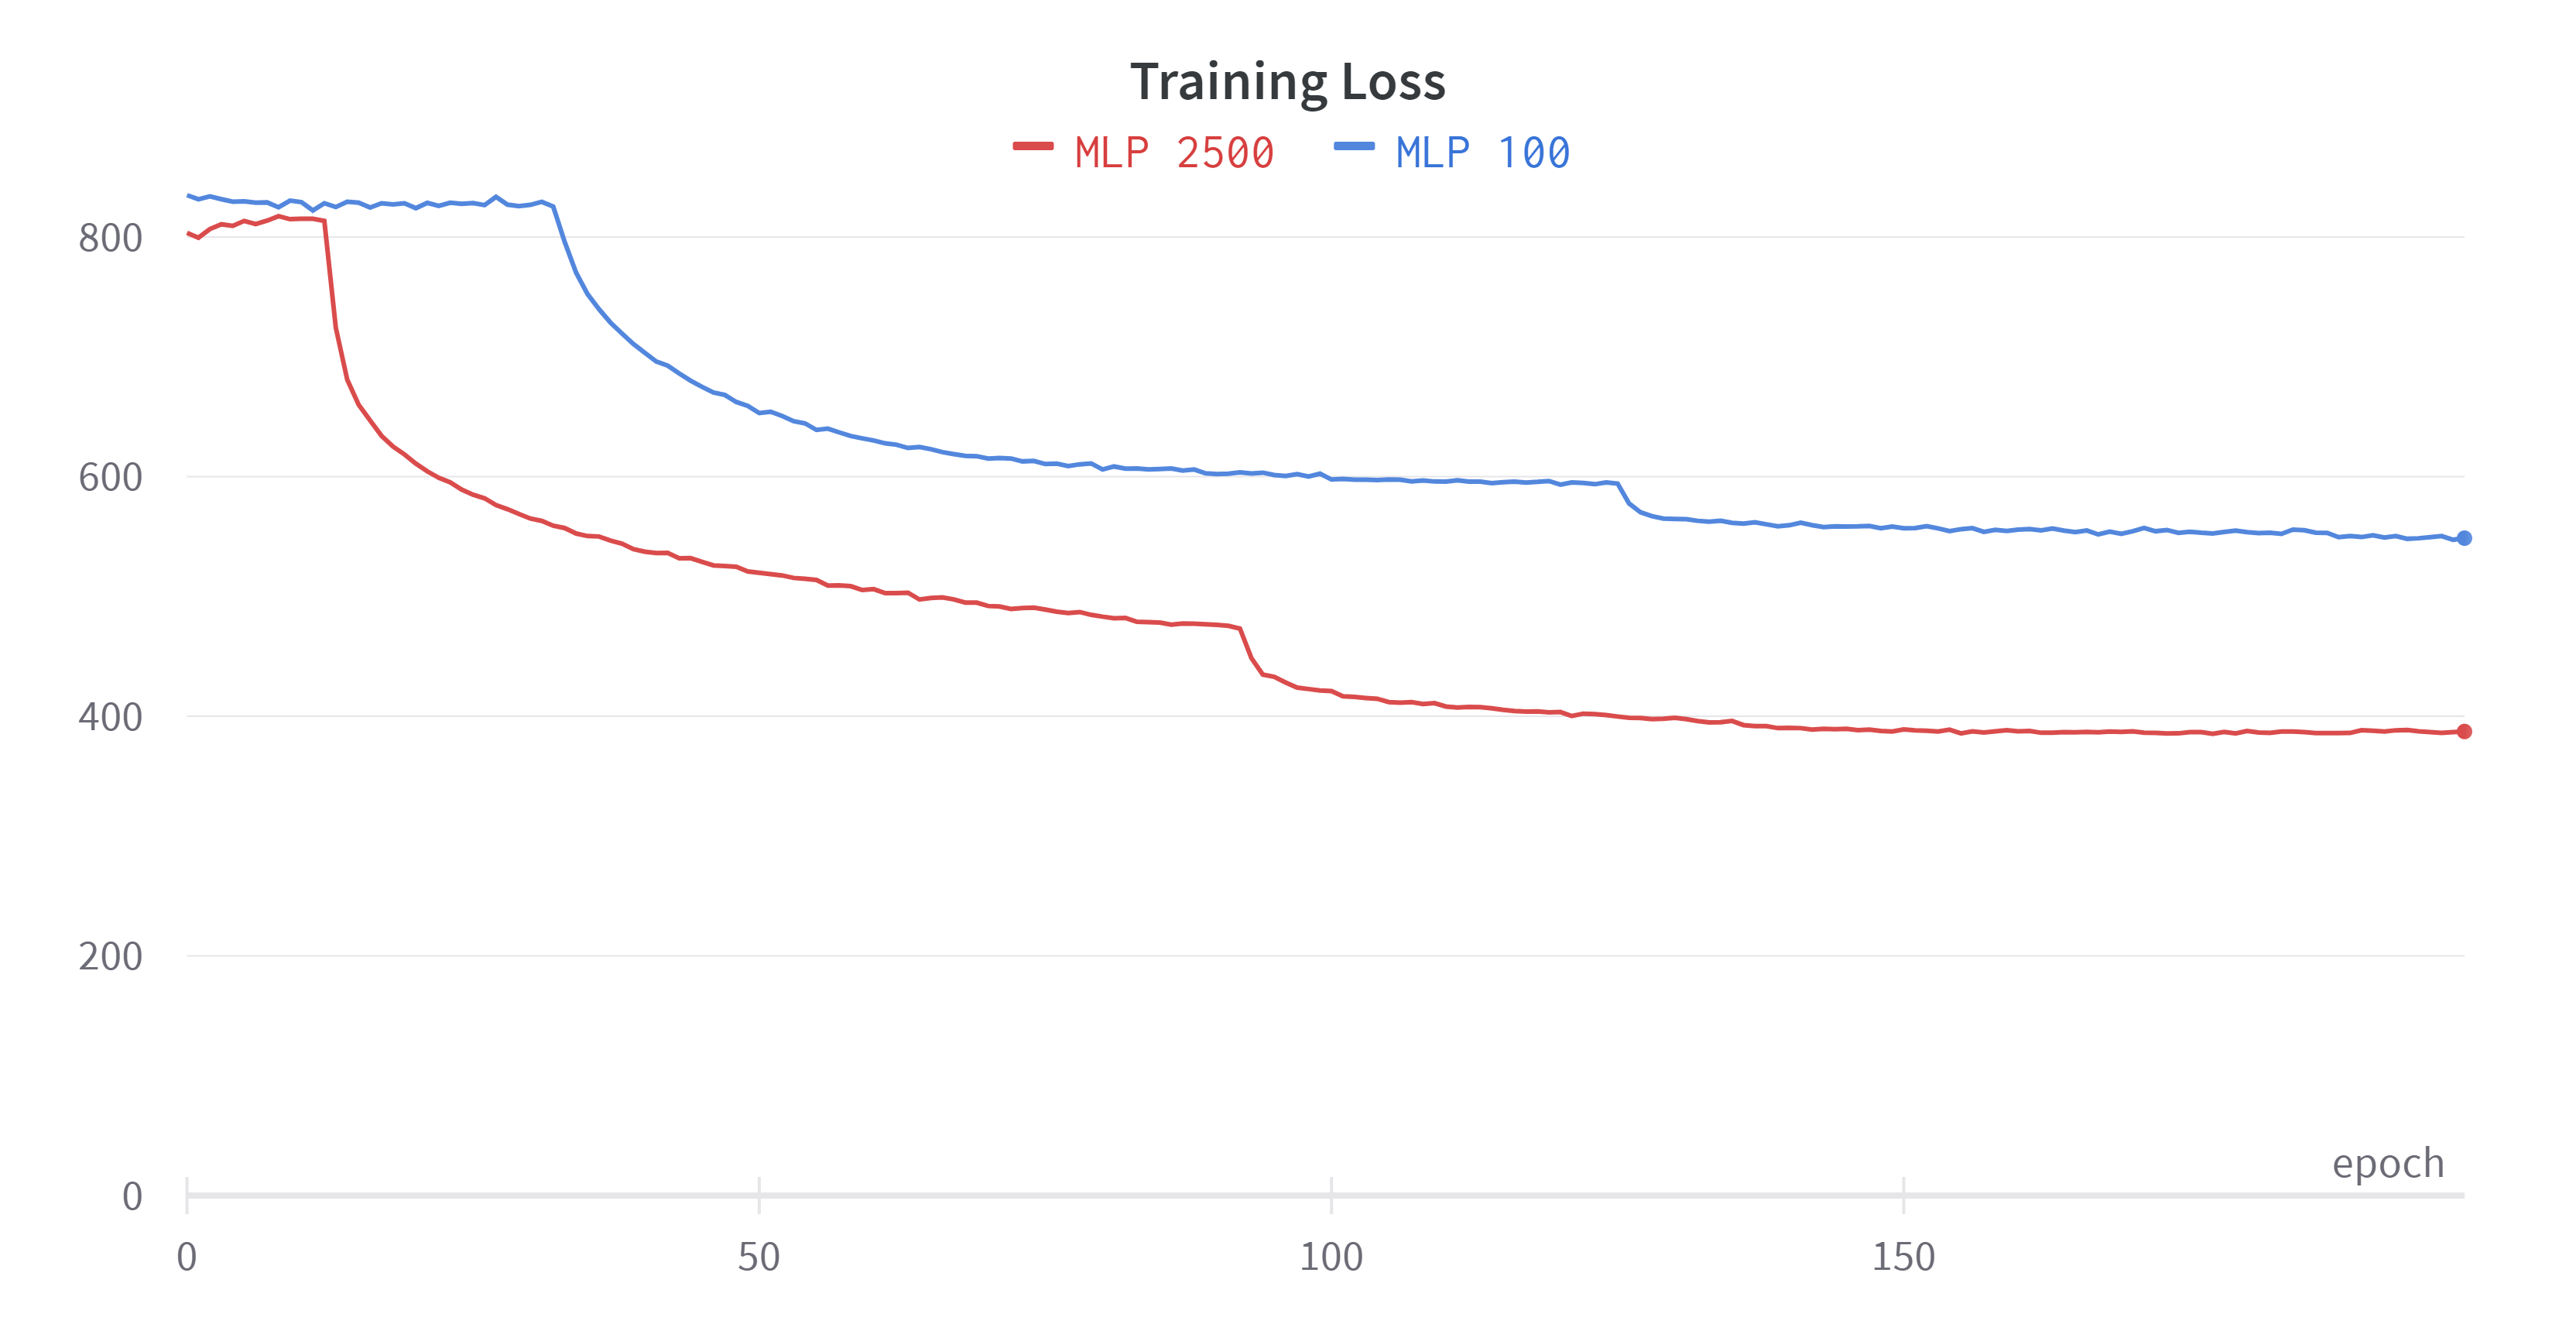
\includegraphics[width=0.9\linewidth]{charts/mlp_cifar_10_train_loss}
\caption{Training loss of two MLP models on CIFAR-10 datasets}
\label{chart: mlp_2}
\end{figure}

\begin{figure}[H]
\centering
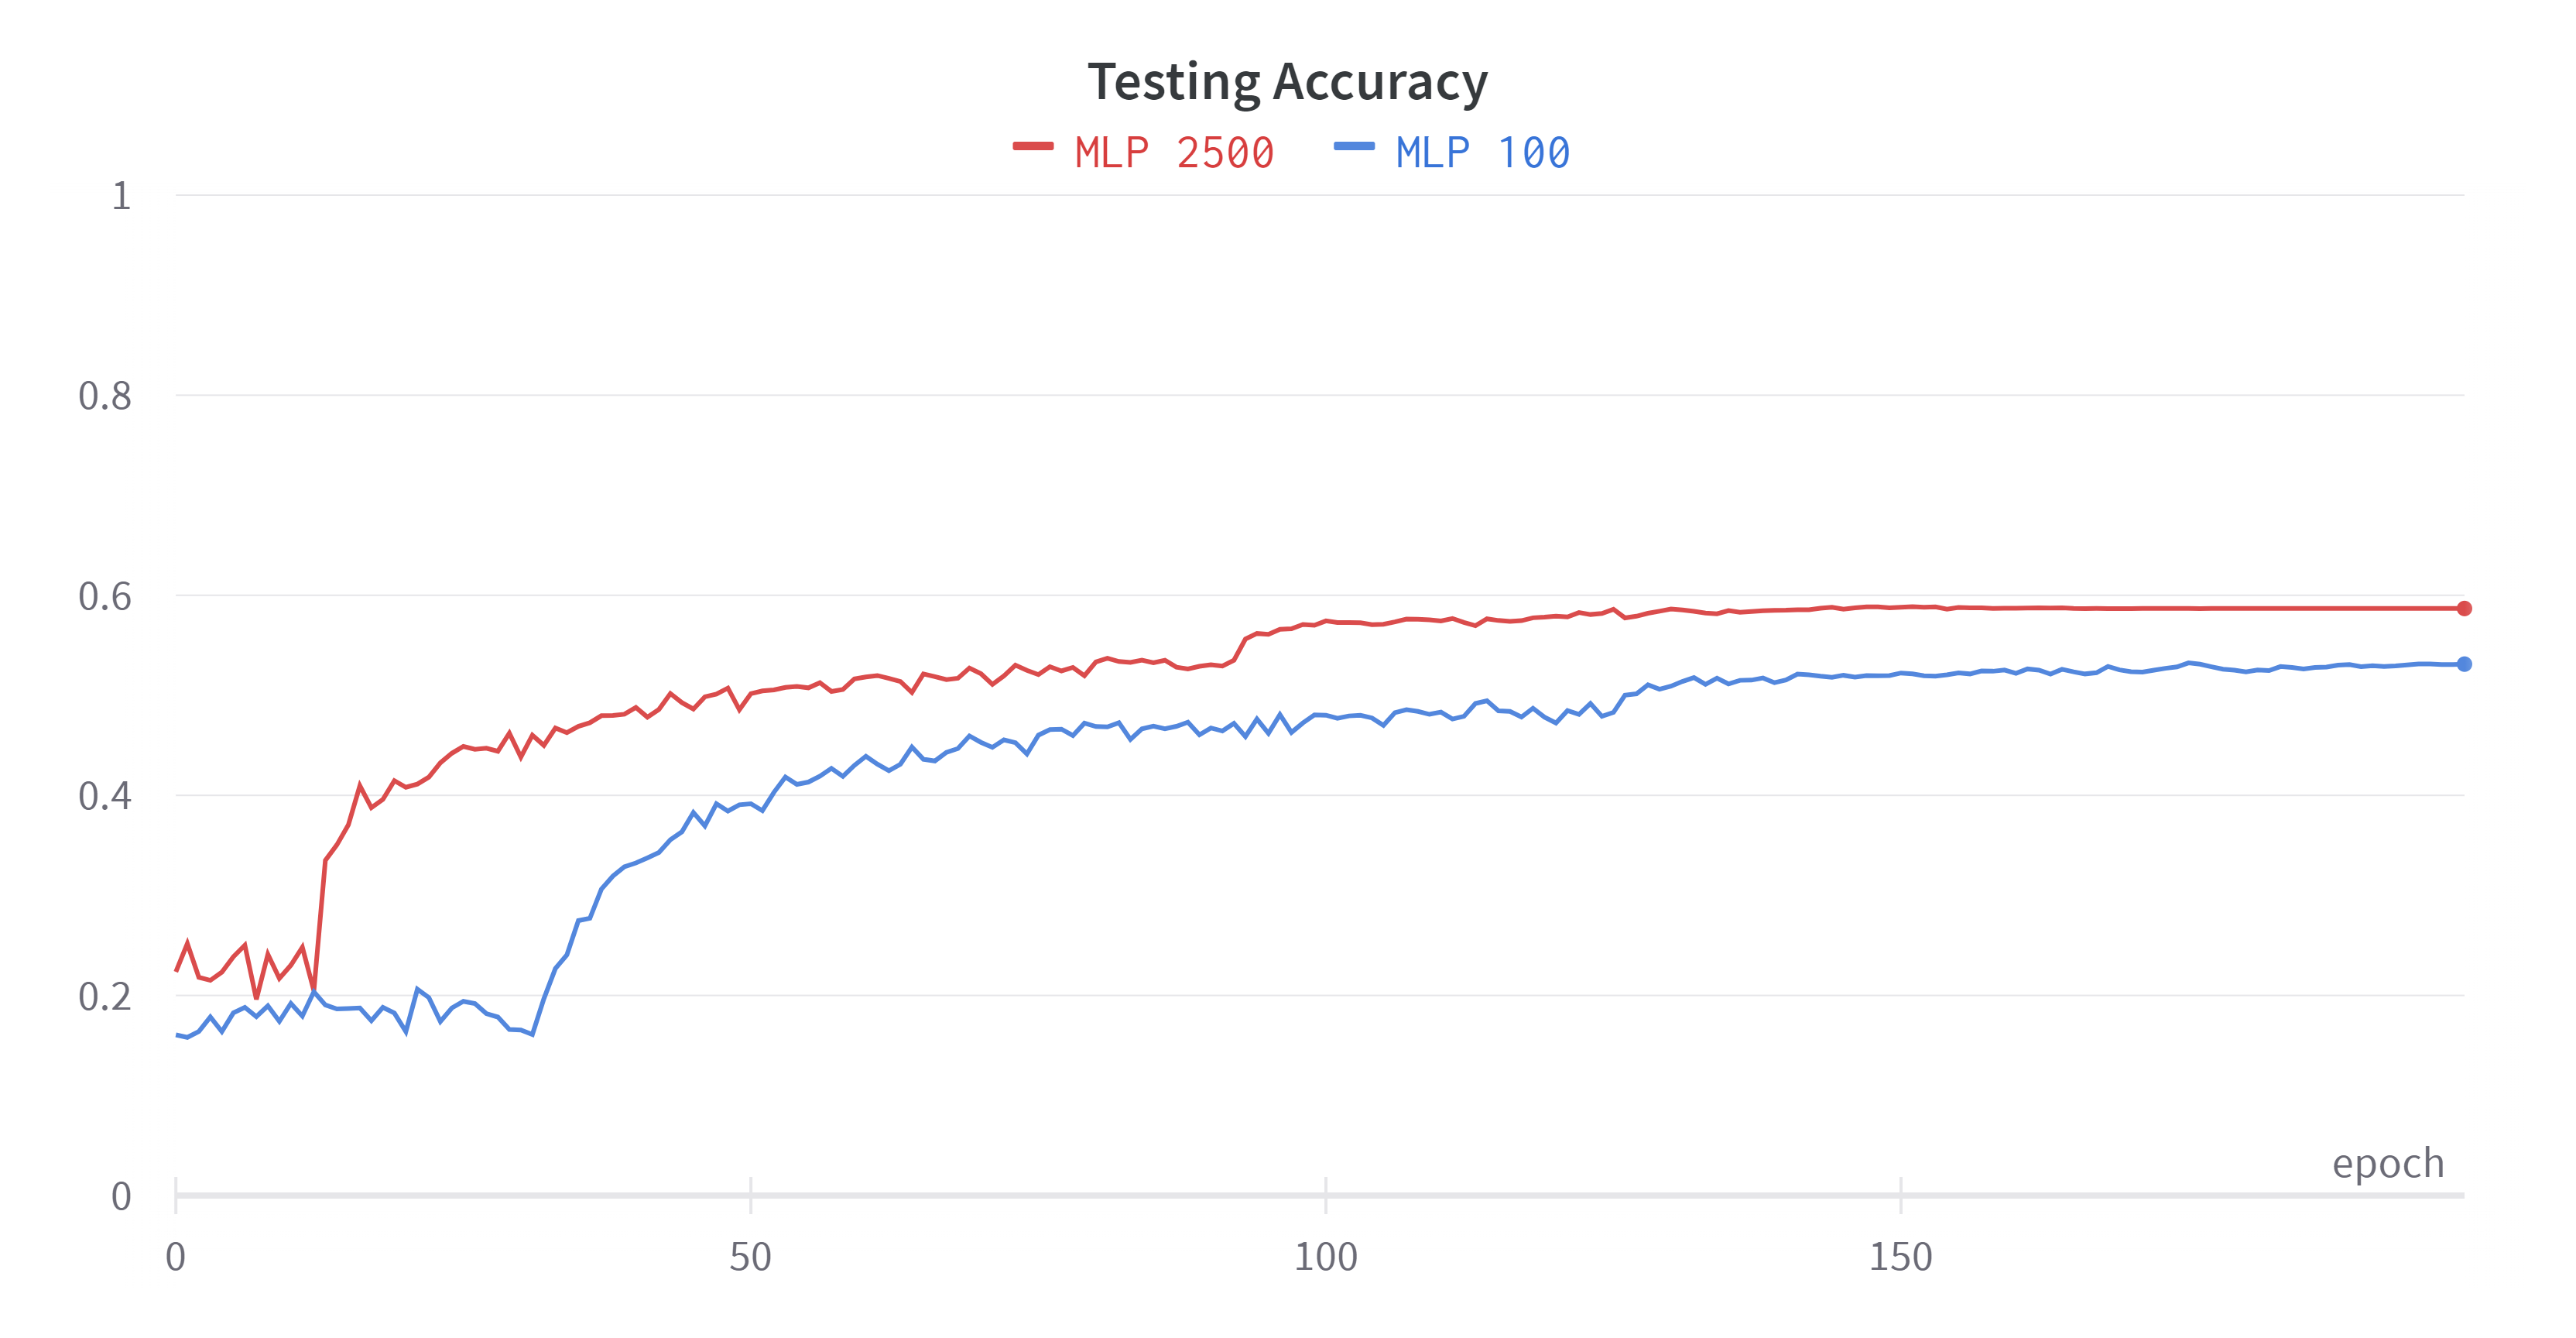
\includegraphics[width=0.9\linewidth]{charts/mlp_cifar_10_test_acc}
\caption{Testing accuracy of two MLP models on CIFAR-10 datasets}
\label{chart: mlp_3}
\end{figure}

\begin{figure}[H]
\centering
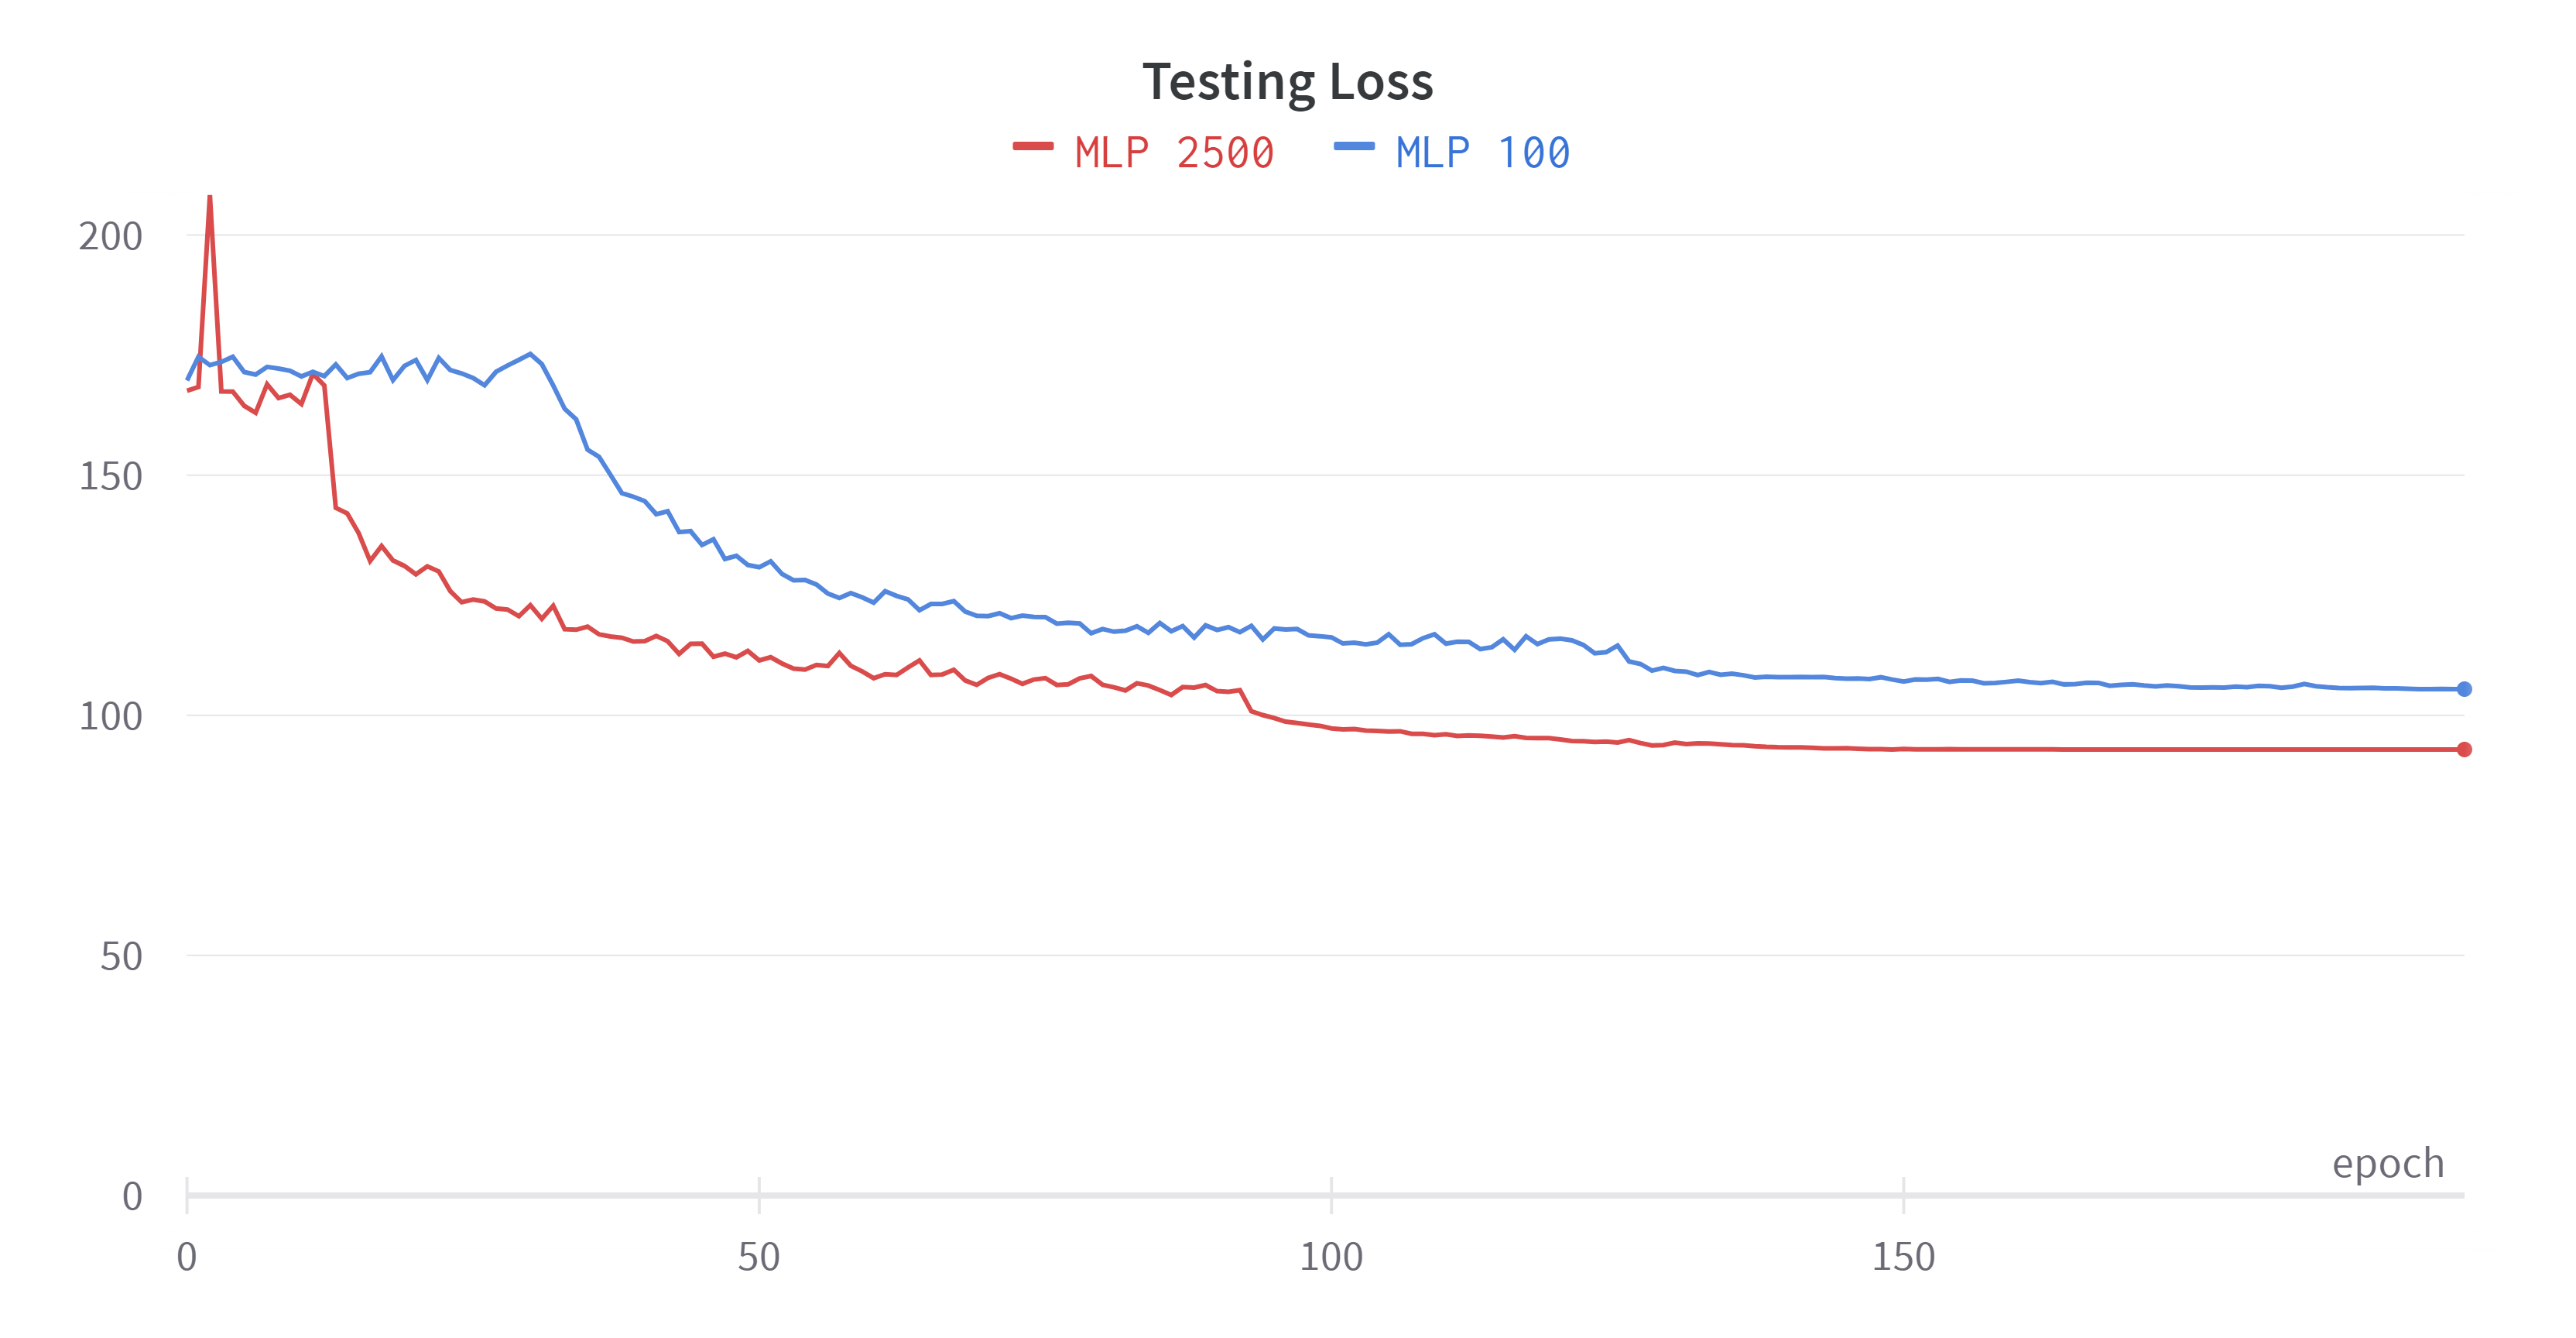
\includegraphics[width=0.9\linewidth]{charts/mlp_cifar_10_test_loss}
\caption{Testing loss of two MLP models on CIFAR-10 datasets}
\label{chart: mlp_4}
\end{figure}


\begin{figure}[H]
\centering
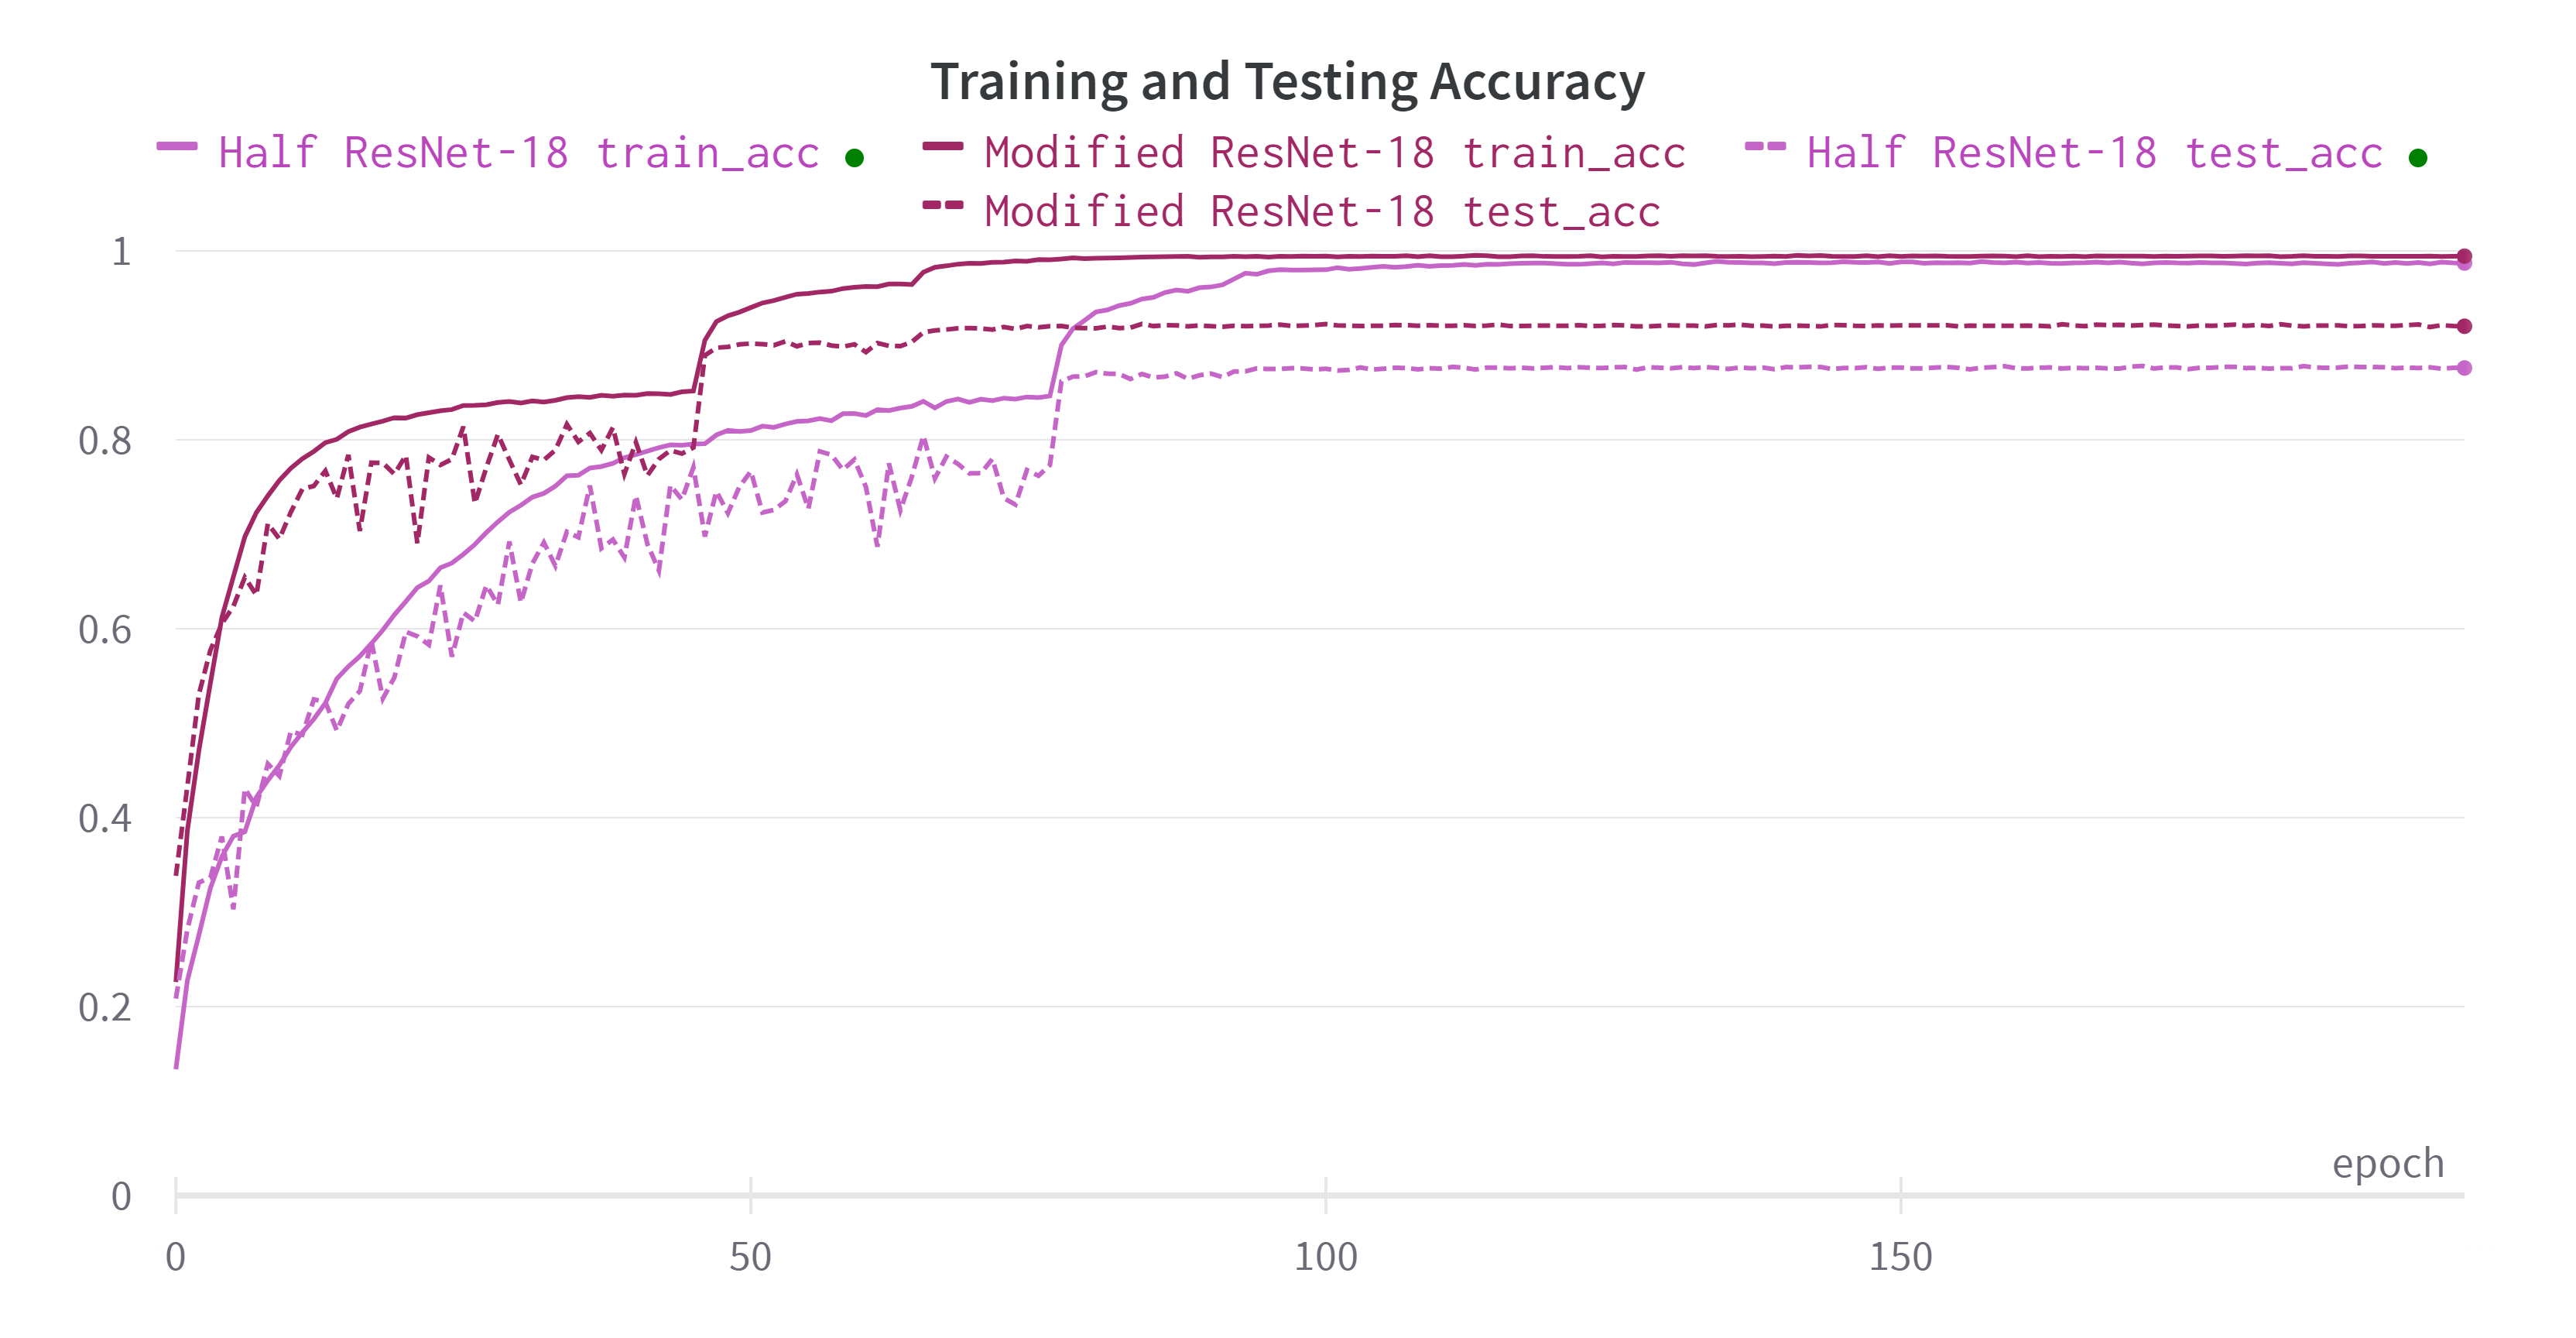
\includegraphics[width=0.9\linewidth]{charts/resnet-half-cifar-acc}
\caption{Training and testing accuracy of ResNet-18 with different training data amount. The ``Half-ResNet-18'' is trained with only 25000 training images.}
\label{fig:resnet-half-cifar-acc}
\end{figure}

\begin{figure}[H]
\centering
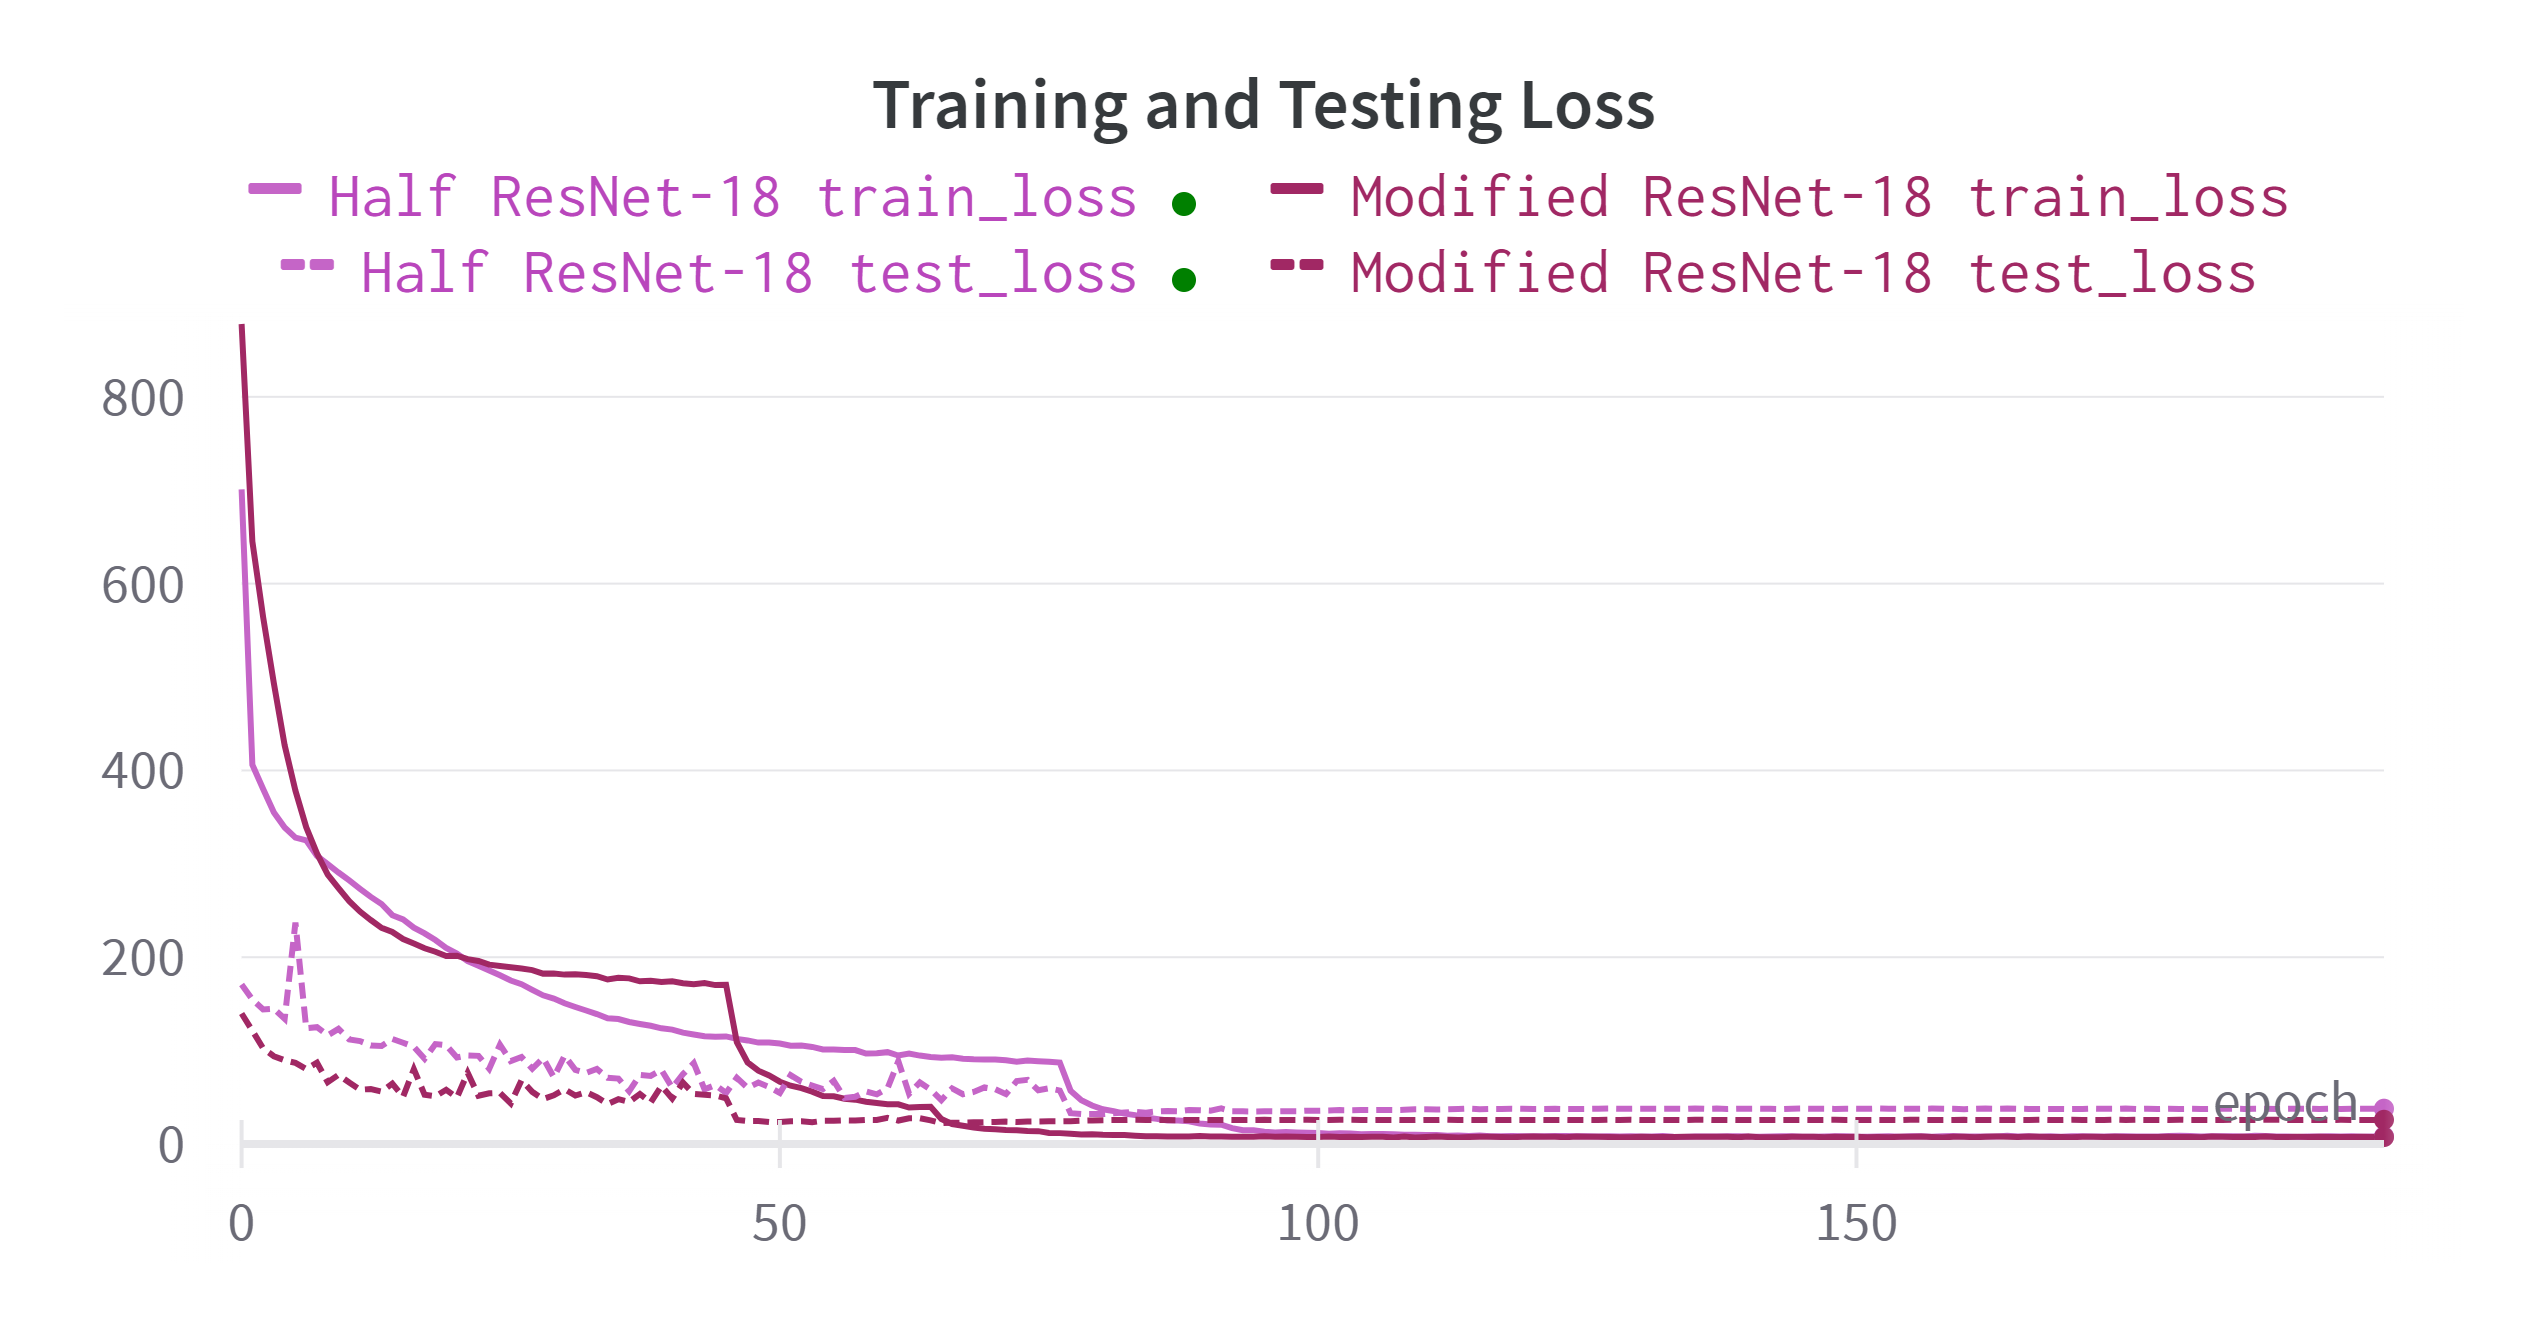
\includegraphics[width=0.9\linewidth]{charts/resnet-half-cifar-loss}
\caption{Training and testing loss of ResNet-18 with different training data amount. The ``Half-ResNet-18'' is trained with only 25000 training images.}
\label{fig:resnet-half-cifar-loss}
\end{figure}

\begin{figure}[H]
\centering
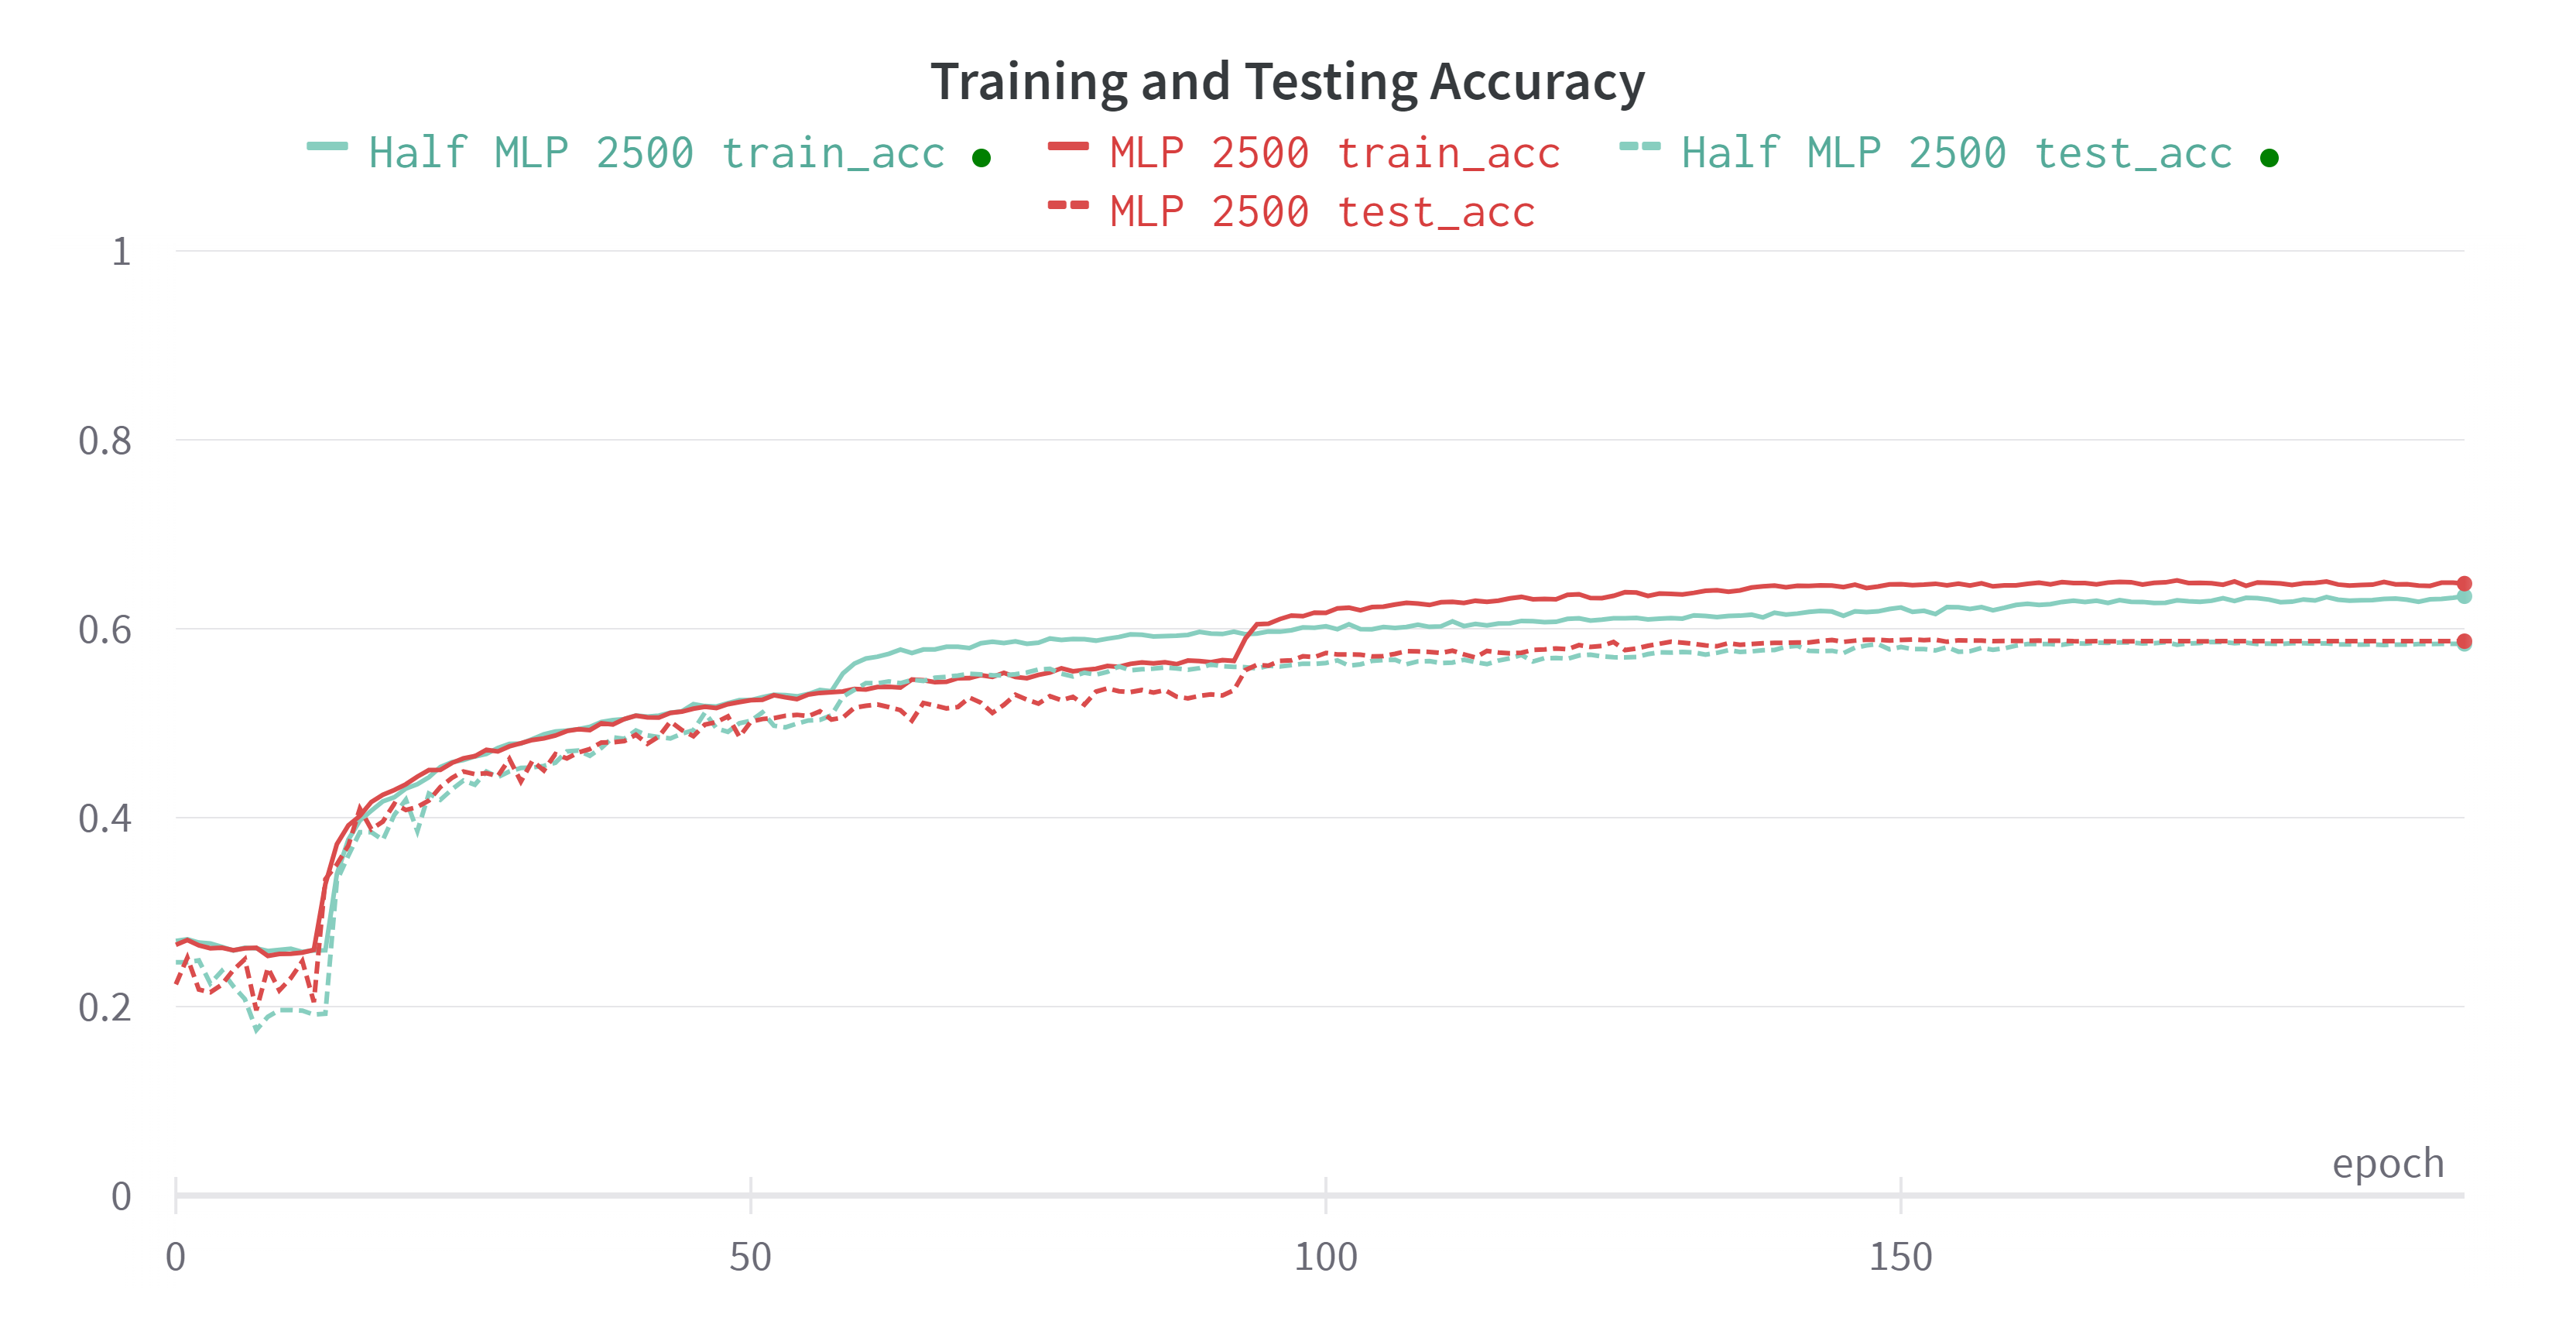
\includegraphics[width=0.9\linewidth]{charts/mlp-half-cifar-acc}
\caption{Training and testing accuracy of MLP with different training data amount. The ``Half MLP'' is trained with only 25000 training images.}
\label{fig:mlp-half-cifar-acc}
\end{figure}

\begin{figure}[H]
\centering
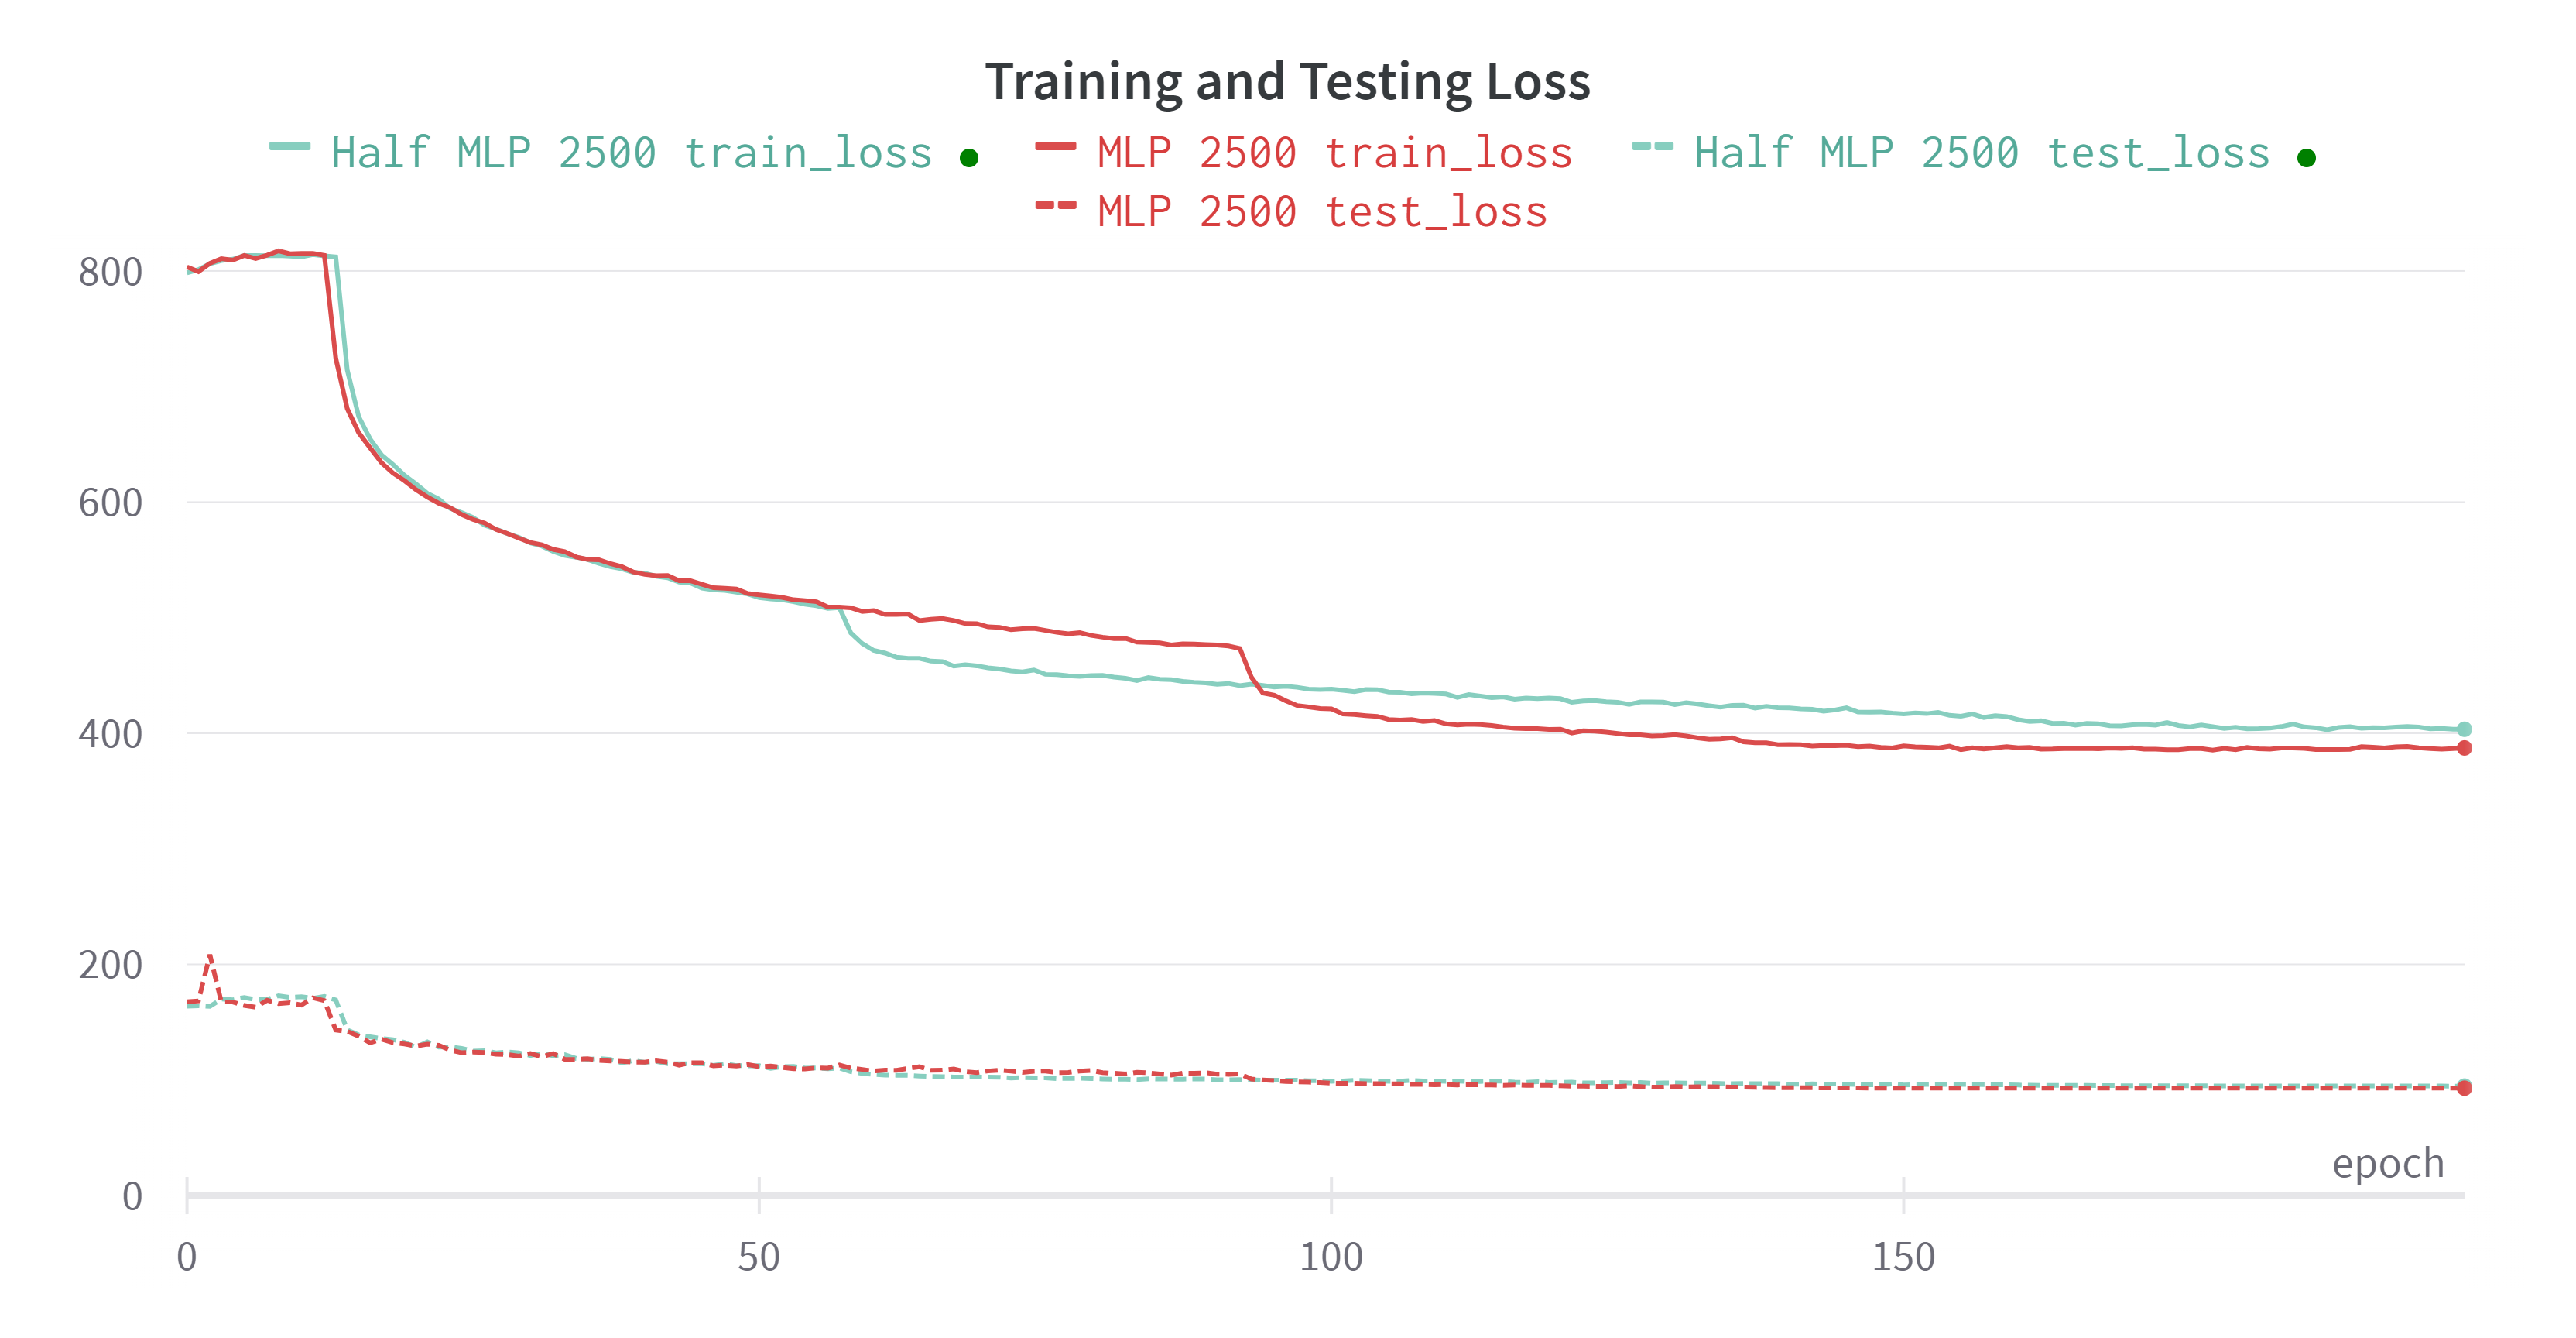
\includegraphics[width=0.9\linewidth]{charts/mlp-half-cifar-loss}
\caption{Training and testing accuracy of MLP with different training data amount. The ``Half MLP'' is trained with only 25000 training images.}
\label{fig:mlp-half-cifar-loss}
\end{figure}


\subsection{Public Non-image Datasets: 20 Newsgroups}

\subsection{Self-mad Datasets: Staellite Images of 5 Regions}

\section{Code of CIFAR-10}
\subsection{Training ResNet-18}
\subsection{Training MLP}
\section{Code of 20 Newsgroups}
\subsection{Training Random Forest Classifier}
\subsection{Training Gradient Boosting Classifier}
\subsection{Training AdaBoost Classifier}
\subsection{Training MLP Classifier}
\section{Code of Satellite Image Datasets}
\subsection{Collect the Images}
\end{appendices}

\end{document}
